\documentclass{article}
\usepackage[preprint]{neurips_2025}

\usepackage[utf8]{inputenc}
\usepackage[T1]{fontenc}
\usepackage{amsmath,amssymb,amsfonts}
\usepackage{graphicx}
\usepackage{booktabs}
\usepackage{hyperref}
\usepackage{xcolor}
\usepackage{microtype}
\usepackage{multirow}
\usepackage{subcaption}
\usepackage{algorithm}
\usepackage{algorithmic}

\hypersetup{
  colorlinks=true,
  linkcolor=blue!60!black,
  citecolor=blue!60!black,
  urlcolor=blue!70!black,
}

\title{Noise-Adaptive Spectral Embedding: Practical Truncation Rules \\ for Diffusion Maps Under Additive Noise}

\author{
  Shreyash Reddy \\
  Department of Data Science \\
  University of California, San Diego \\
  \texttt{DSC 205 --- Winter 2026}
}

\begin{document}

\maketitle

% ============================================================================
\begin{abstract}
Diffusion maps and Laplacian eigenmaps embed high-dimensional point clouds into low-dimensional representations by retaining leading eigenvectors of a graph operator. The number of retained eigenvectors---the spectral truncation point---is critical: too few discard structure, too many embed noise. The noisy-Laplacian theory predicts that the transition between signal and noise eigenvectors occurs at an index scaling as $C/r^2$, where $r$ is the noise standard deviation and $C$ is a geometry-dependent constant. However, neither $C$ nor $r$ is available in practice.

We implement and evaluate three data-driven truncation strategies on five synthetic manifolds across 120 seeded experiment runs: (i)~a \emph{bandwidth-stability} rule that identifies signal modes by their invariance to kernel bandwidth perturbations, (ii)~a \emph{noise-amplitude-based} cutoff that estimates $r$ from nearest-neighbor distances and applies $k^* = \lfloor C/r^2 \rfloor$, and (iii)~the standard \emph{eigengap} heuristic. Bandwidth stability produces noise-adaptive, seed-consistent cutoffs on manifolds with uniform curvature---on the circle, the cutoff decreases monotonically from $k{=}8$ to $k{=}4$ as noise increases eight-fold, with zero seed variance---and outperforms the eigengap by $+3.5$ percentage points in trustworthiness on the S-curve. The method fails on the Swiss roll due to eigenvector reordering across bandwidths. The kNN noise estimator systematically conflates manifold geometry with noise, underestimating $r$ on the circle ($0.3$--$0.7\times$ true) and overestimating on the Swiss roll ($2$--$7\times$), confirming the fundamental difficulty of noise estimation from nearest-neighbor distances. We validate estimator accuracy against the empirical noise standard deviation computed directly from the known noise vectors, providing ground truth tighter than the configured noise parameter.
\end{abstract}

% ============================================================================
\section{Introduction}
\label{sec:intro}

Spectral methods for nonlinear dimensionality reduction---diffusion maps~\citep{coifman2006diffusion}, Laplacian eigenmaps~\citep{belkin2003laplacian}, and their variants---construct a weighted graph from pairwise point similarities and embed data via the leading eigenvectors of the resulting graph operator. A central decision in these methods is \emph{how many eigenvectors to keep}. Retaining too few eigenvectors discards manifold structure; retaining too many includes eigenvectors that are dominated by noise and carry no geometric information.

The \emph{eigengap heuristic}, which selects $k$ at the largest drop between consecutive eigenvalues, is the standard approach~\citep{vonluxburg2007tutorial}. It works when the spectrum has a sharp cliff separating signal from noise, but on many manifolds the eigenvalue decay is gradual and the largest gap can shift with different random seeds.

Recent theoretical work on noisy graph Laplacians~\citep{elkaroui2016connection} formalizes a threshold phenomenon: when $n$ points are sampled from a smooth $d$-dimensional manifold in $\mathbb{R}^D$ with additive Gaussian noise of standard deviation $r$, the graph Laplacian eigenvectors split into two regimes. The first ${\sim}\, C/r^2$ eigenvectors approximate the manifold's Laplacian eigenfunctions, while those beyond this index are noise-dominated. The constant $C$ depends on the manifold's intrinsic geometry (curvature and reach).

In principle, knowledge of $r$ and $C$ would yield the ideal truncation point $k^* = C/r^2$. In practice, neither is available. This project investigates two practical alternatives. First, following course feedback suggesting that signal eigenvectors should remain stable across bandwidth perturbations while noise modes should not, we implement a \emph{bandwidth-stability truncation} rule. Second, we implement and evaluate a direct noise-estimation approach using $k$-nearest-neighbor distances, testing whether the theoretical formula can be made practical with an estimated $r$ and an empirically calibrated $C$.

\paragraph{Informal statement of the main theoretical result.}
Consider $n$ points sampled uniformly from a smooth, compact $d$-dimensional manifold $\mathcal{M} \subset \mathbb{R}^D$, corrupted by additive isotropic Gaussian noise with variance $r^2$. Form the graph Laplacian with an appropriately chosen bandwidth. Then eigenvectors with index up to approximately $C(\mathcal{M})/r^2$ converge (as $n \to \infty$) to the manifold Laplacian's eigenfunctions. Beyond this index, eigenvectors are noise-dominated. The constant $C(\mathcal{M})$ encodes intrinsic geometric properties: manifolds with higher curvature or smaller reach have smaller $C$, meaning fewer modes survive at a given noise level.

\paragraph{Course feedback and project evolution.}
Our initial proposal aimed to estimate $r$ from kNN distances and compute $k^* = C/r^2$ directly. The professor's feedback identified three key challenges: (1)~nearest-neighbor distances conflate noise with manifold geometry, making $r$-estimation non-trivial; (2)~the constant $C$ reflects curvature and reach, so it cannot be easily computed; (3)~bandwidth stability offers a practical alternative that sidesteps both problems. Based on this feedback, we restructured the project into phases: Phase~1 implements bandwidth stability and comparison experiments on synthetic manifolds; Phase~2a integrates Levina--Bickel intrinsic dimension estimation; Phase~2b validates the $r^{-2}$ scaling law using oracle data; Phase~2c implements kNN noise estimation and the $r$-based cutoff formula, evaluating it honestly against both bandwidth stability and the eigengap.

% ============================================================================
\section{Background}
\label{sec:background}

\subsection{Diffusion Maps}

Given $n$ points $\{x_i\}_{i=1}^n \subset \mathbb{R}^D$, we construct a diffusion-map embedding as follows~\citep{coifman2006diffusion}:
\begin{enumerate}
    \item Compute pairwise squared distances and form the Gaussian affinity matrix $W_{ij} = \exp\!\bigl(-\|x_i - x_j\|^2 / \varepsilon\bigr)$.
    \item Apply $\alpha$-normalization ($\alpha = 0.5$) to correct for non-uniform sampling density: $K_\alpha = D^{-\alpha} W D^{-\alpha}$, where $D$ is the diagonal degree matrix~\citep{coifman2006diffusion}.
    \item Row-normalize to obtain the diffusion operator $P = \tilde{D}^{-1} K_\alpha$.
    \item Compute the leading eigenpairs $\{(\lambda_j, \psi_j)\}_{j=0}^{K}$ of $P$.
    \item Embed point $x_i$ as $\bigl(\lambda_1^t \psi_1(i),\;\lambda_2^t \psi_2(i),\;\ldots,\;\lambda_k^t \psi_k(i)\bigr)$, where $t$ is the diffusion time.
\end{enumerate}
The convergence of the graph Laplacian to the manifold Laplacian is well-established~\citep{singer2006graph, belkin2003laplacian}. However, this convergence applies only to the signal eigenvectors. Under additive noise, eigenvectors beyond the $C/r^2$ threshold do not converge to any geometric quantity~\citep{elkaroui2016connection}.

\subsection{Why Bandwidth Stability Works in Principle}

Perturbing the bandwidth $\varepsilon$ changes the diffusion operator. Geometric eigenvectors---those corresponding to manifold structure---are determined by the manifold and should be relatively insensitive to moderate bandwidth changes, at least within a range bounded by the manifold's reach~\citep{berry2016variable, niyogi2008finding}. Noise-dominated eigenvectors, which depend on scale-specific fluctuations, should vary substantially. Cross-bandwidth agreement thus serves as a proxy for distinguishing signal from noise without requiring estimation of $C$ or $r$.

% ============================================================================
\section{Methods}
\label{sec:methods}

\subsection{Eigengap Heuristic (Baseline)}

The eigengap method computes gaps $g_k = \lambda_k - \lambda_{k+1}$ over a configured range $[\text{min}_k, \text{max}_k]$ and returns the $k$ with the largest gap~\citep{vonluxburg2007tutorial}. It is simple and well-understood, but on many manifolds the decay is gradual, the gap is small or non-unique, and the selected $k$ can jump across random seeds.

\subsection{Bandwidth-Stability Cutoff}
\label{sec:bandwidth_stability}

Our primary method is described in Algorithm~\ref{alg:stability}. For each mode index $k$, we measure the absolute inner product between the $k$-th normalized eigenvector at adjacent bandwidths, then average across all adjacent pairs. Modes with mean stability at or above a threshold $\tau$ (default 0.9) are retained as signal.

\begin{algorithm}[htbp]
\caption{Bandwidth-Stability Truncation}
\label{alg:stability}
\begin{algorithmic}[1]
\REQUIRE Noisy point cloud $X$, bandwidth grid $\{\varepsilon_1, \ldots, \varepsilon_B\}$, threshold $\tau$
\FOR{$b = 1, \ldots, B$}
    \STATE Build diffusion operator $P^{(b)}$ at bandwidth $\varepsilon_b$
    \STATE Compute leading $K$ eigenvectors $\{\psi_1^{(b)}, \ldots, \psi_K^{(b)}\}$
\ENDFOR
\FOR{each mode index $k = 1, \ldots, K$}
    \STATE $\displaystyle s(k) \leftarrow \frac{1}{B-1} \sum_{b=1}^{B-1} \bigl|\langle \hat{\psi}_k^{(b)},\; \hat{\psi}_k^{(b+1)} \rangle\bigr|$
\ENDFOR
\RETURN $k^* = \max\{k : s(k) \geq \tau\}$
\end{algorithmic}
\end{algorithm}

If no mode meets the threshold, the method falls back to $k = \text{min}_k$. The choice of $\tau$ is analyzed empirically in Section~\ref{sec:threshold_sensitivity}.

\subsection{Oracle Cutoff (Synthetic-Only Benchmark)}

For synthetic data where clean manifold points are available, we compute the $k$ that minimizes the chordal subspace distance between the span of the first $k$ clean eigenvectors and the first $k$ noisy eigenvectors~\citep{elkaroui2016connection}. This is not usable in practice but provides a gold-standard reference for how well any method could recover the clean eigenspace.

\subsection{Intrinsic Dimension Estimation}

We integrated the Levina--Bickel maximum-likelihood estimator~\citep{levina2004maximum} for intrinsic dimension. For each point, it computes a local dimension estimate from the ratio of successive neighbor distances, then averages across all points. The estimate serves as an independent diagnostic: it gives a data-driven reference for how many dimensions the manifold has, which helps interpret whether truncation cutoffs are retaining a reasonable number of modes.

\subsection{Noise Amplitude Estimation}
\label{sec:noise_est_methods}

We implement two kNN-based noise estimators. For data $X = M + \text{noise}$ with noise $\sim \mathcal{N}(0, r^2 I_D)$, the expected squared distance between nearby points satisfies:
\begin{equation}
\mathbb{E}\bigl[\|x_i - x_j\|^2\bigr] = \|m_i - m_j\|^2 + 2Dr^2
\label{eq:expected_distance}
\end{equation}
where $D$ is the ambient dimension. At the nearest-neighbor scale, the manifold term $\|m_i - m_j\|^2$ is assumed small relative to the noise term $2Dr^2$. In practice, this assumption is violated to varying degrees depending on the manifold geometry.

\paragraph{Simple estimator.} Uses the median $k$-th nearest-neighbor squared distance:
\begin{equation}
\hat{r}_{\text{simple}}^2 = \frac{\mathrm{median}(d_k^2)}{2D}
\label{eq:simple_estimator}
\end{equation}

\paragraph{Two-scale estimator.} Uses distances at two neighborhood ranks $k_1 < k_2$ to subtract the manifold contribution, under the heuristic assumption that the manifold term scales linearly with $k$:
\begin{equation}
\hat{r}_{\text{2-scale}}^2 = \frac{k_2 \cdot \overline{d_{k_1}^2} - k_1 \cdot \overline{d_{k_2}^2}}{(k_2 - k_1) \cdot 2D}
\label{eq:twoscale_estimator}
\end{equation}

\subsection{Empirical Noise Amplitude from Data}
\label{sec:empirical_r_method}

Since we use synthetic manifolds where both clean points $X_{\text{clean}}$ and noisy points $X_{\text{noisy}}$ are available, we can compute the realized noise standard deviation directly:
\begin{equation}
r_{\text{empirical}} = \mathrm{std}\bigl(X_{\text{noisy}} - X_{\text{clean}}\bigr)
\label{eq:empirical_r}
\end{equation}
This provides a tighter ground truth than the configured noise parameter $r$. While $r$ describes the distribution from which noise was drawn, $r_{\text{empirical}}$ captures the exact noise realization in each run. For our sample sizes ($n = 450$, $D = 3$--$5$), $r_{\text{empirical}} / r_{\text{configured}}$ falls in $[0.976, 1.009]$, confirming data generation accuracy and providing a precise benchmark for evaluating the kNN estimators.

\subsection{r-Based Cutoff}
\label{sec:r_based_cutoff}

Given an estimate of $r$ (either known or estimated) and a geometry constant $C$ (calibrated from oracle data), we compute:
\begin{equation}
k^* = \left\lfloor \frac{C}{r^2} \right\rfloor, \quad \text{clipped to } [\text{min}_k,\; \text{max}_k]
\label{eq:r_based}
\end{equation}
We test two modes: \emph{known-$r$}, which uses the true noise standard deviation for validation, and \emph{estimated-$r$}, which applies the kNN estimator on the noisy data alone (the realistic scenario).

\subsection{Evaluation Metrics}

We evaluate embedding quality using three complementary metrics:
\begin{itemize}
    \item \textbf{Trustworthiness}~\citep{venna2001neighborhood}: the fraction of $k$-nearest neighbors in the embedding that are also neighbors in the original space. Measures whether the embedding introduces false neighbors.
    \item \textbf{Continuity}: the fraction of $k$-nearest neighbors in the original space preserved in the embedding. Sensitive to over- or under-dimensioning.
    \item \textbf{Geodesic consistency}: Spearman rank correlation between embedding distances and approximate geodesic distances computed via kNN shortest paths~\citep{tenenbaum2000global}. Measures global structure preservation.
\end{itemize}
Trustworthiness tends to be high even for large $k$ (adding dimensions rarely creates false neighbors), while continuity is more sensitive to the embedding dimension. Geodesic consistency captures whether the embedding preserves the manifold's global geometry beyond just local neighborhoods.

% ============================================================================
\clearpage
\section{Experimental Setup}
\label{sec:setup}

\subsection{Synthetic Manifolds}

All experiments use synthetic point-cloud data generated from five manifolds with controlled additive Gaussian noise (Table~\ref{tab:manifolds}). Points are sampled uniformly on the manifold in native coordinates, zero-padded to ambient dimension $D$, rotated by a deterministic random orthogonal matrix, and corrupted by isotropic Gaussian noise with standard deviation $r$. Figure~\ref{fig:manifold_panels} shows each manifold at increasing noise levels, visualized via PCA projection of the ambient-space data with coordinates fit on the clean points for consistency.

\begin{table}[htbp]
\caption{Synthetic manifolds used in experiments. $d$ is the intrinsic dimension, $D$ is the ambient dimension.}
\label{tab:manifolds}
\centering
\begin{tabular}{@{}lccl@{}}
\toprule
Manifold & $d$ & $D$ & Description \\
\midrule
Circle     & 1 & 3 & Unit circle embedded in $\mathbb{R}^3$ via random rotation \\
Sphere     & 2 & 5 & Unit 2-sphere in $\mathbb{R}^5$ \\
Swiss roll & 2 & 3 & Spiral surface with non-uniform curvature \\
S-curve    & 2 & 3 & S-shaped surface with gradual spectral decay \\
Torus      & 2 & 5 & Flat torus ($R{=}2$, $r_{\text{tube}}{=}0.5$) in $\mathbb{R}^5$ \\
\bottomrule
\end{tabular}
\end{table}

\begin{figure}[htbp]
\centering
\begin{subfigure}[b]{0.98\textwidth}
    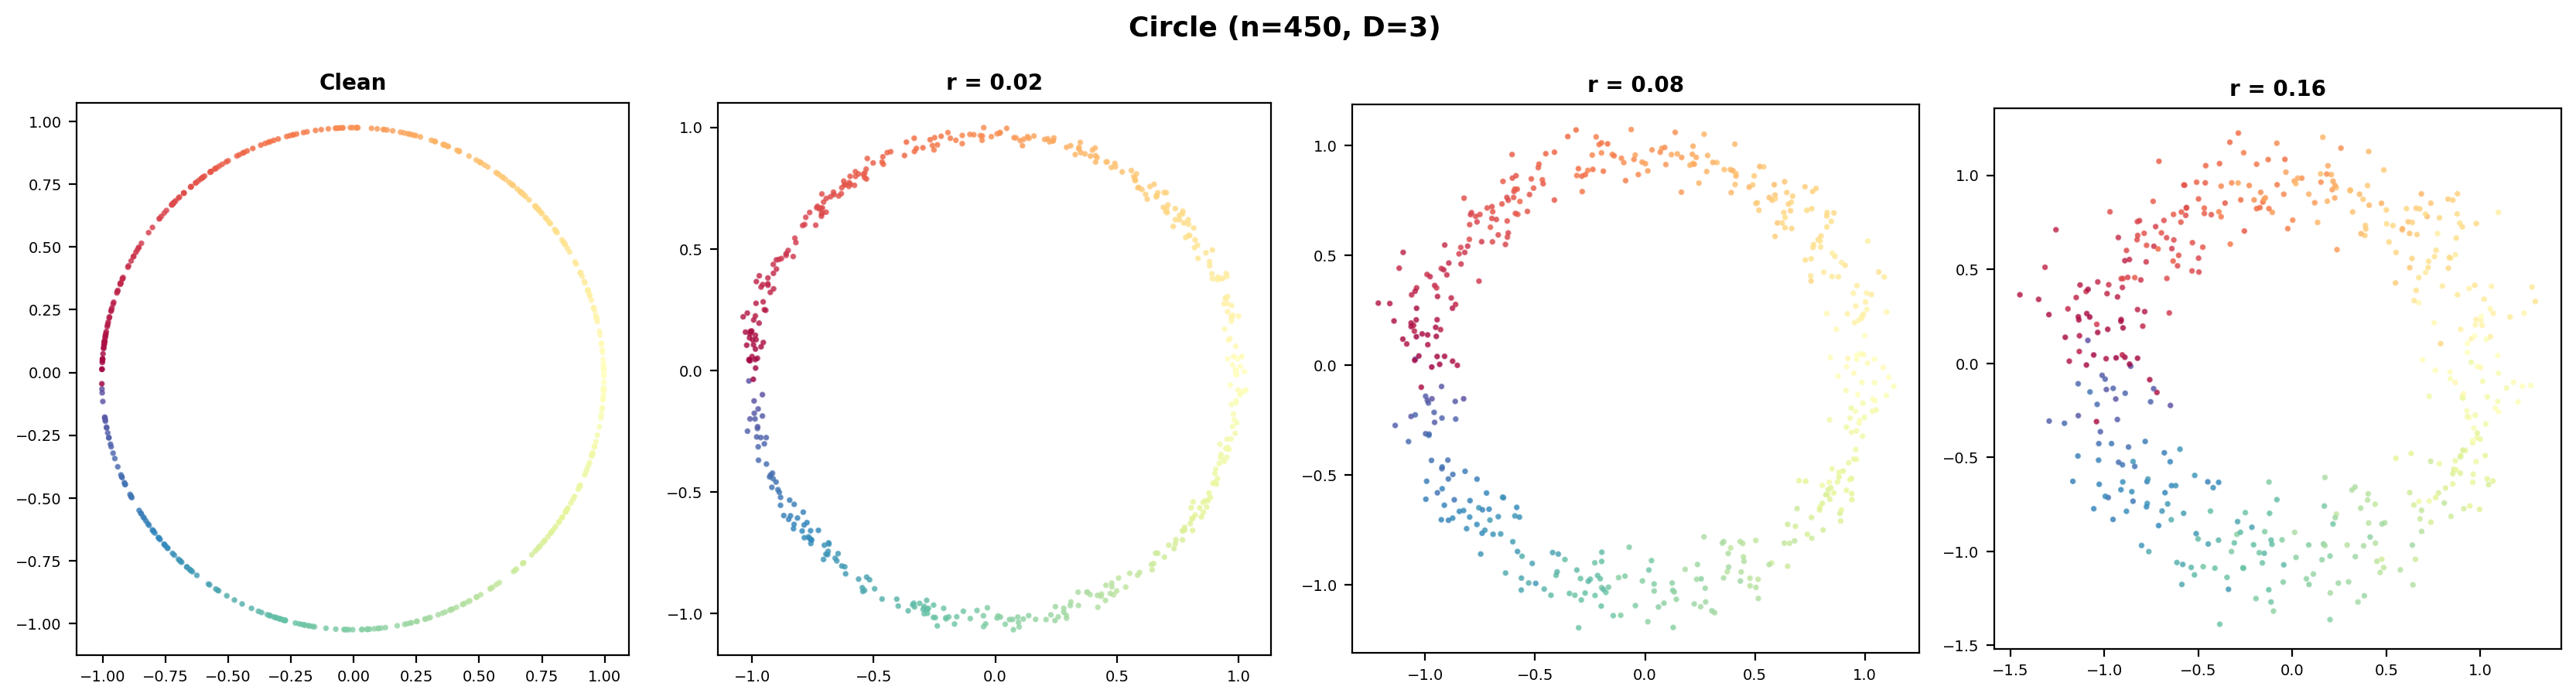
\includegraphics[width=\textwidth]{figures/circle_noise_panel.png}
\end{subfigure}
\vspace{1mm}
\begin{subfigure}[b]{0.98\textwidth}
    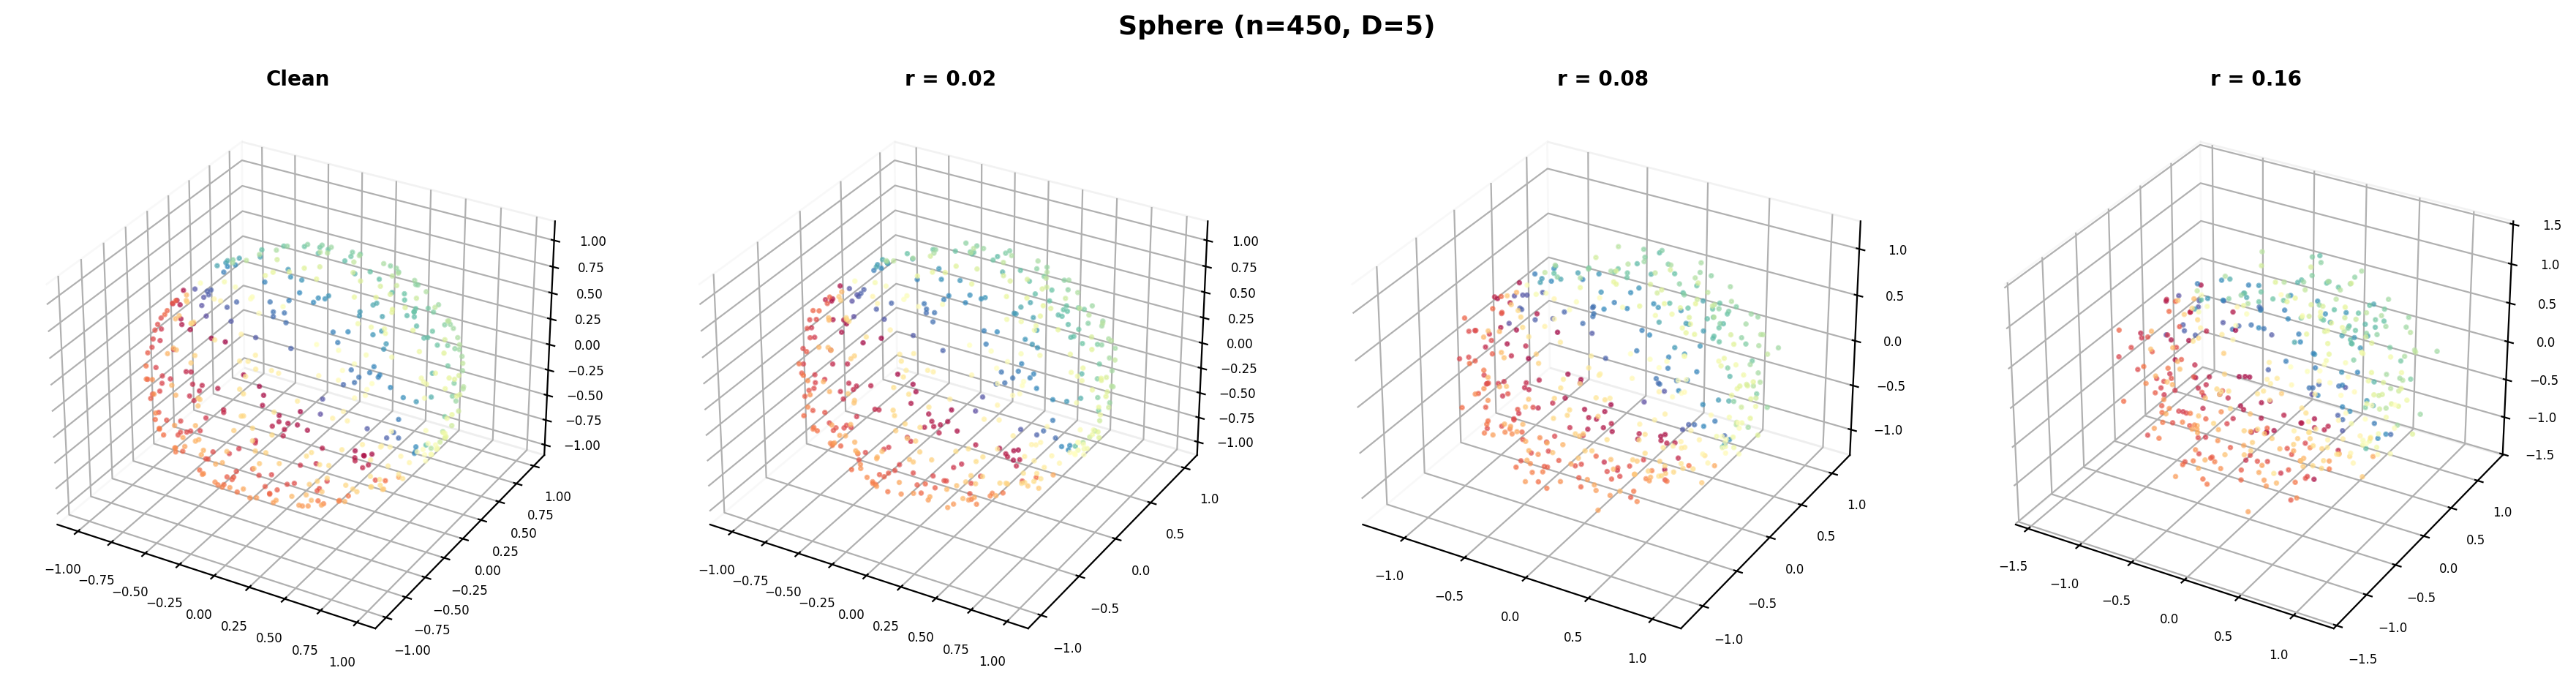
\includegraphics[width=\textwidth]{figures/sphere_noise_panel.png}
\end{subfigure}
\vspace{1mm}
\begin{subfigure}[b]{0.98\textwidth}
    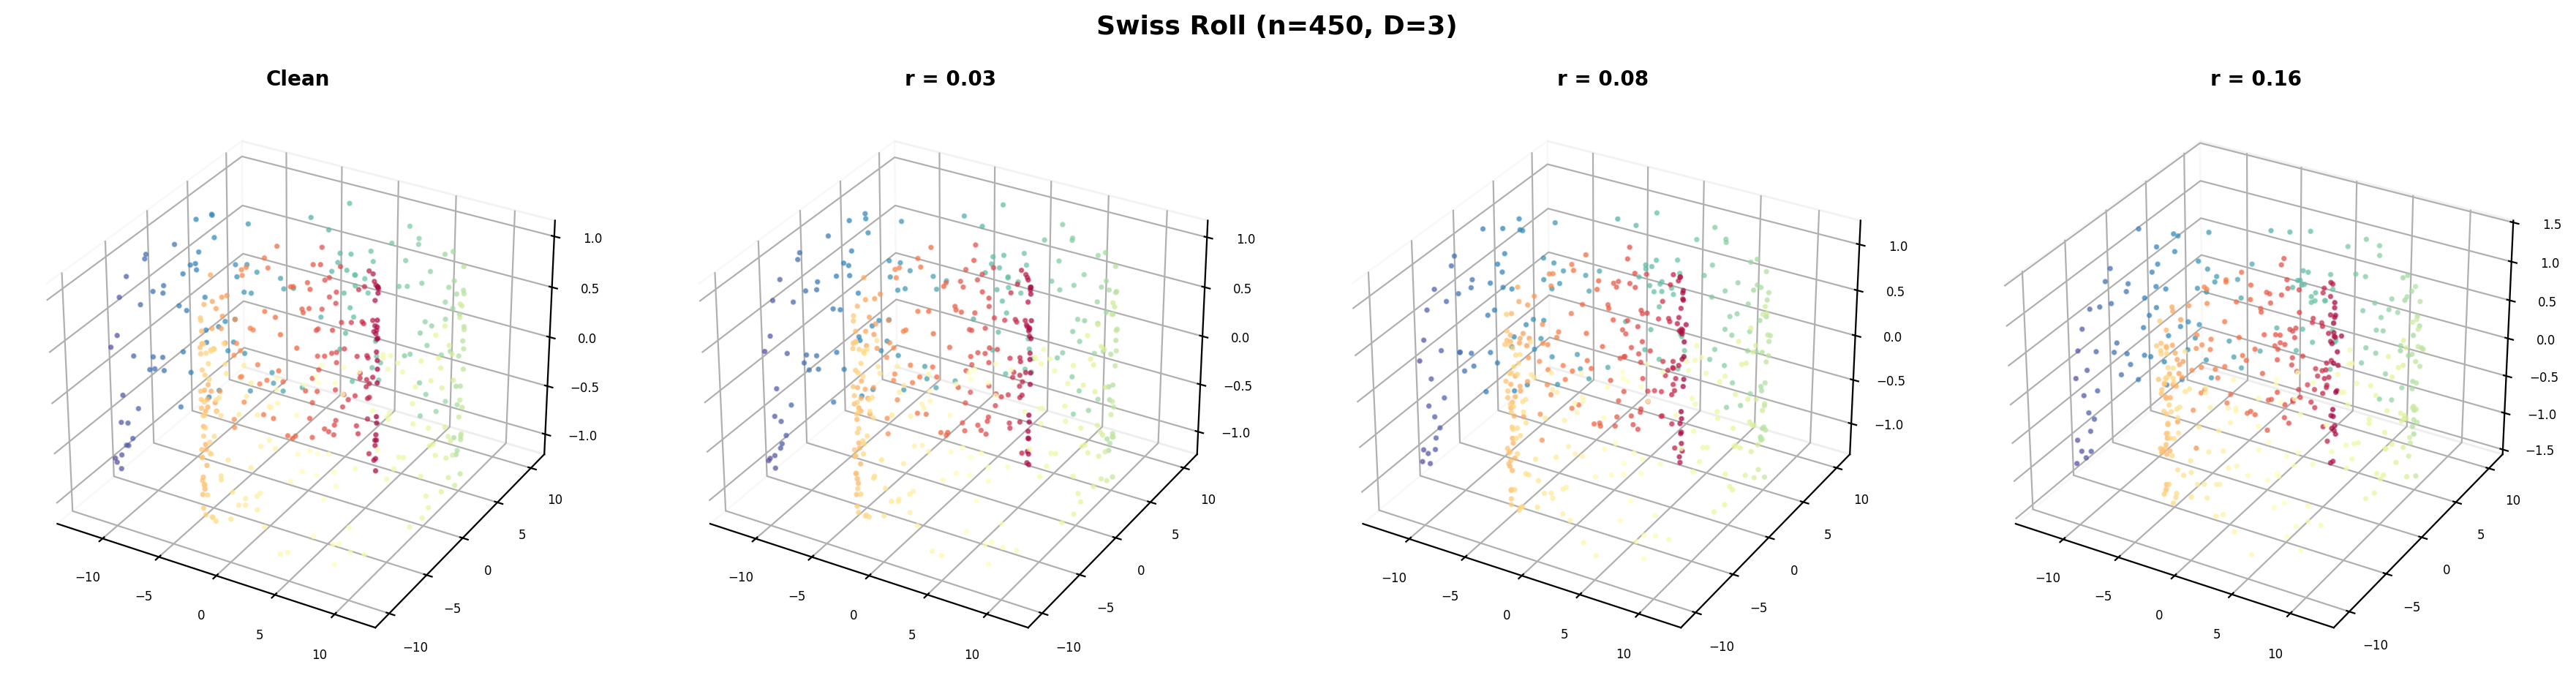
\includegraphics[width=\textwidth]{figures/swiss_roll_noise_panel.png}
\end{subfigure}
\vspace{1mm}
\begin{subfigure}[b]{0.98\textwidth}
    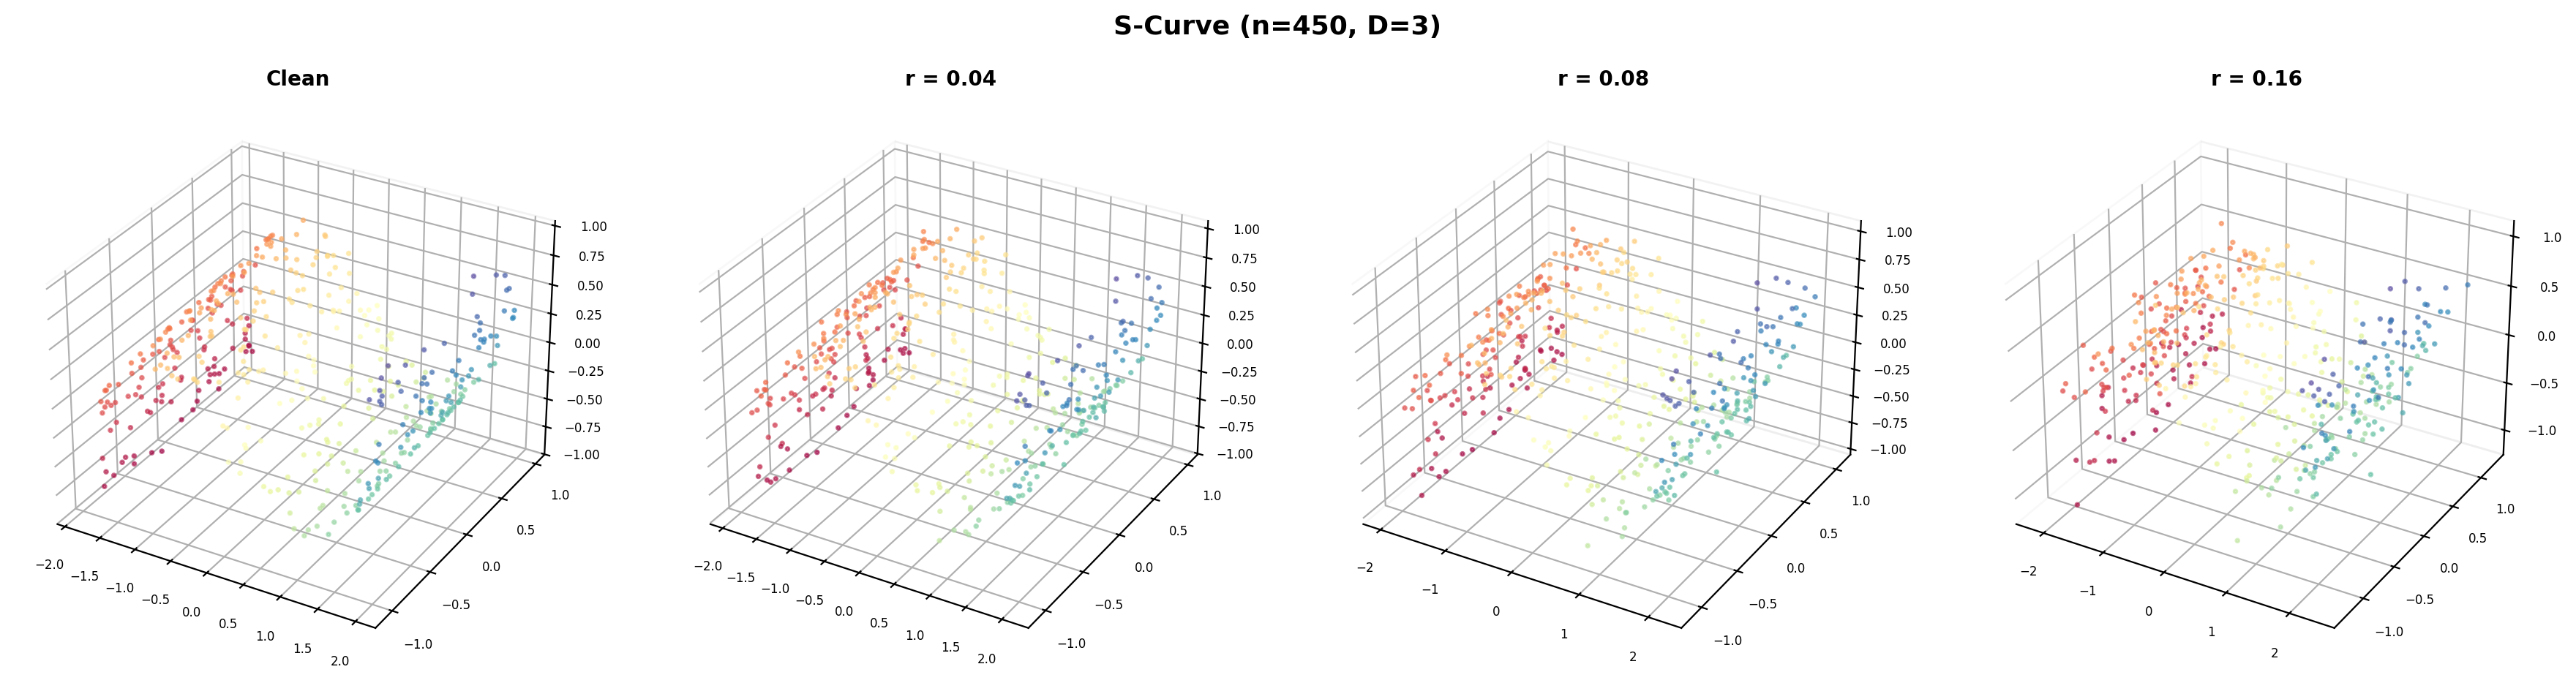
\includegraphics[width=\textwidth]{figures/s_curve_noise_panel.png}
\end{subfigure}
\vspace{1mm}
\begin{subfigure}[b]{0.98\textwidth}
    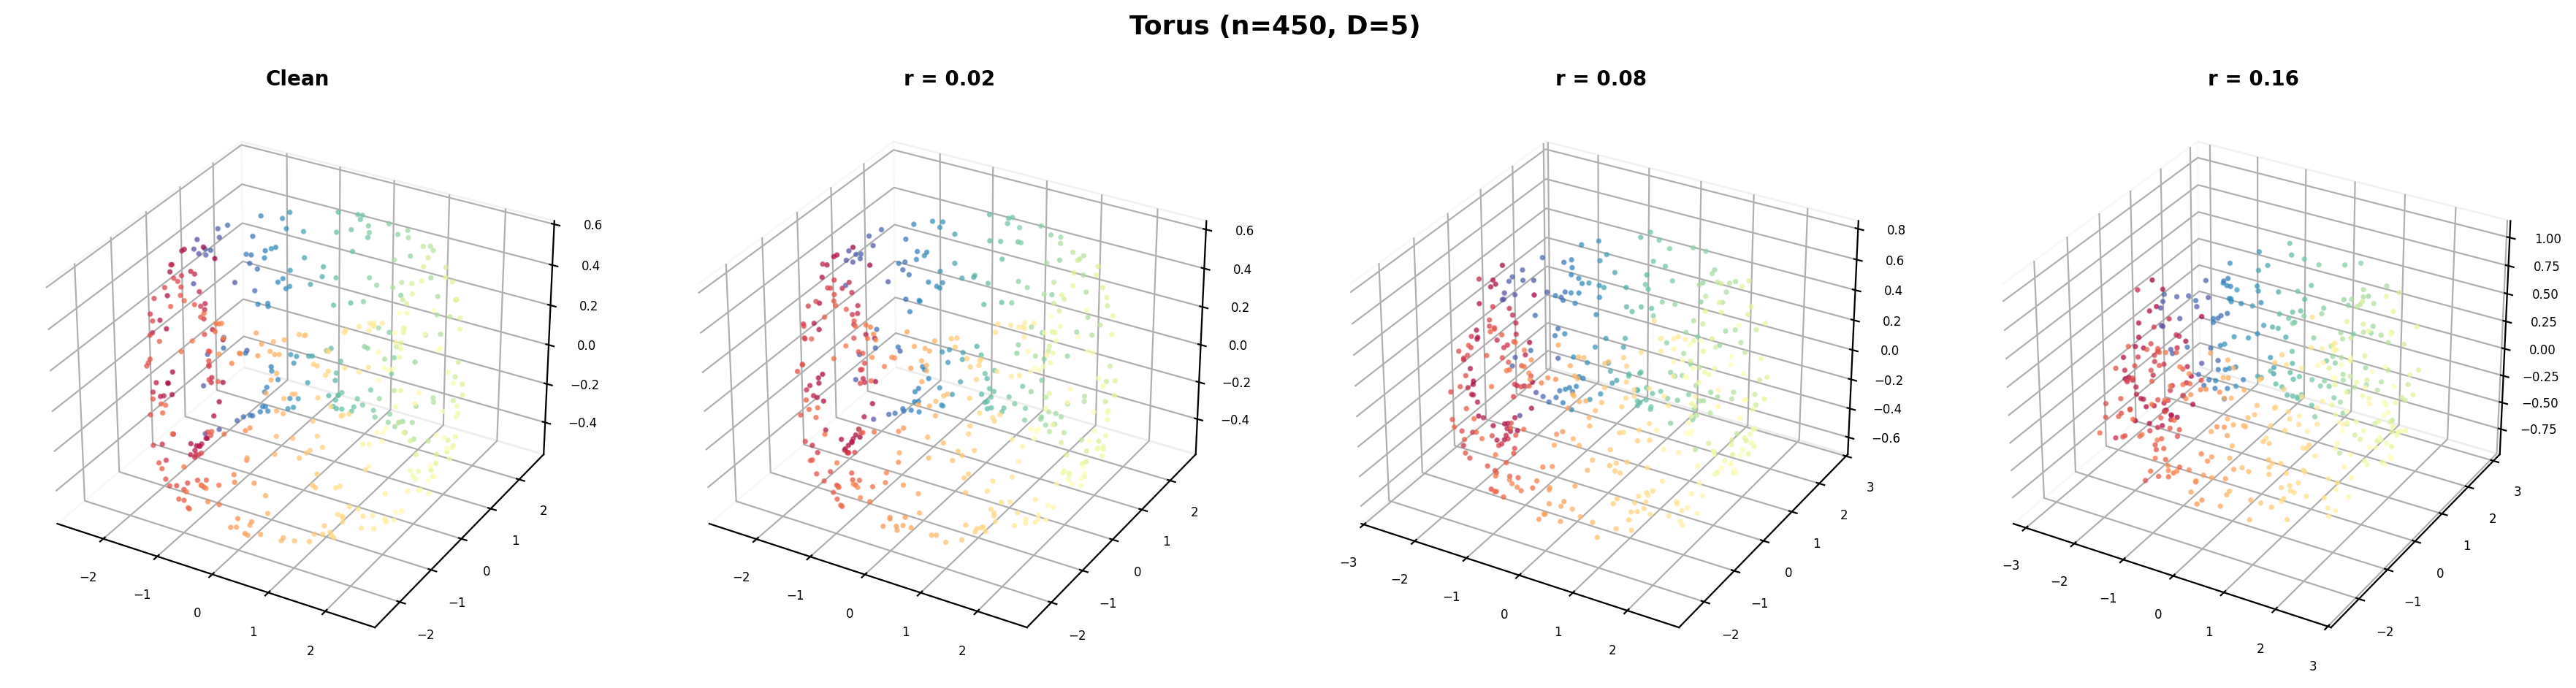
\includegraphics[width=\textwidth]{figures/torus_noise_panel.png}
\end{subfigure}
\caption{All five synthetic manifolds at increasing noise levels (left to right: clean, low noise, medium noise, high noise). Points are colored by a latent parameter. PCA coordinates are fit on the clean data and applied to all noisy versions so the degradation is visible in a consistent frame.}
\label{fig:manifold_panels}
\end{figure}

\subsection{Experiment Inventory}

We conducted 120 experiment runs across 12 configurations, organized in two phases (Table~\ref{tab:experiments}). Phase~1 evaluates bandwidth stability and eigengap on all five manifolds under controlled noise. Phase~2c implements and tests the noise-estimation pipeline and the $r$-based cutoff formula.

\begin{table}[htbp]
\caption{Full experiment inventory. Each sweep runs across all listed noise levels and seeds.}
\label{tab:experiments}
\centering
\small
\begin{tabular}{@{}cllcccr@{}}
\toprule
Phase & Config & Manifold(s) & $n$ & Noise $r$ & Seeds & Runs \\
\midrule
1 & noise\_sweep\_circle\_sphere & Circle, Sphere & 450 & 0.02/0.08/0.16 & 3 & 18 \\
1 & synthetic\_noise\_sweep & Swiss roll & 400 & 0.03/0.08/0.16 & 3 & 9 \\
1 & ambiguous\_gap\_suite & S-curve & 500 & 0.12 & 3 & 6 \\
1 & eigengap\_ambiguous\_suite & Sphere ($D{=}6$) & 450 & 0.14 & 3 & 6 \\
1 & threshold\_sensitivity & Circle & 450 & 0.08 & 3 & 12 \\
1 & torus\_noise\_sweep & Torus & 450 & 0.02/0.08/0.16 & 3 & 9 \\
1 & bandwidth\_sweep & Swiss roll & 400 & 0.08 & 2 & 4 \\
\midrule
2c & r\_estimation\_circle\_sphere & Circle, Sphere & 450 & 0.02--0.16 & 3 & 30 \\
2c & r\_validation\_known\_r & Circle, Sphere & 450 & 0.02/0.08/0.16 & 3 & 18 \\
2c & r\_estimation\_swiss\_roll & Swiss roll & 400 & 0.03/0.08/0.16 & 2 & 6 \\
\midrule
& & & & & \textbf{Total:} & \textbf{120} \\
\bottomrule
\end{tabular}
\end{table}

\subsection{Reproducibility}

All experiments are controlled by YAML configuration files with deterministic seeding via a single \texttt{numpy.random.Generator}. Each run produces a timestamped directory containing the exact config snapshot, all computed metrics in JSON format, serialized arrays (embeddings, eigenvalues, eigenvectors, stability scores), and generated figures. The full experiment suite can be reproduced from the repository:
\begin{verbatim}
pip install -e .[dev]
nase sweep --config configs/noise_sweep_circle_sphere.yaml
python3 scripts/analyze_results.py
\end{verbatim}

% ============================================================================
\clearpage
\section{Results: Bandwidth Stability}
\label{sec:results_stability}

\subsection{Circle: Noise-Adaptive Cutoff with Zero Seed Variance}

The circle--sphere noise sweep provides the strongest evidence for bandwidth stability. On the circle ($n = 450$, $D = 3$), the cutoff decreases monotonically with noise and is perfectly consistent across seeds (Table~\ref{tab:circle_results}).

\begin{table}[htbp]
\caption{Circle: full metrics across noise levels (3-seed means).}
\label{tab:circle_results}
\centering
\begin{tabular}{@{}ccccccc@{}}
\toprule
$r$ & $k_{\text{stab}}$ ($\pm$std) & $k_{\text{gap}}$ & $k_{\text{oracle}}$ & Trust. & Cont. & Geo.\ cons. \\
\midrule
0.02 & 8.0 $\pm$ 0.0 & 2 & 1.3 & 0.9997 & 0.885 & 0.778 \\
0.08 & 6.0 $\pm$ 0.0 & 2 & 1.3 & 0.993 & 0.584 & 0.770 \\
0.16 & 4.0 $\pm$ 0.0 & 2 & 1.3 & 0.981 & 0.453 & 0.746 \\
\bottomrule
\end{tabular}
\end{table}

The stability profile (Figure~\ref{fig:stability_circle}) reveals a sharp boundary between signal and noise modes. At $r = 0.02$, modes 1--8 have stability scores above 0.999, while mode~9 drops sharply. At $r = 0.16$, the boundary shifts to mode~4, with mode~5 dropping to 0.847. This is exactly the behavior predicted by the noisy-Laplacian theory: more noise corrupts more modes, and the stability metric detects this boundary precisely.

The eigengap always selects $k = 2$ (the gap after the cosine--sine pair), regardless of noise level. It cannot adapt because the spectral gap structure of the circle does not change with noise---the leading eigenvalues remain separated, and only the eigenvectors beyond the gap change character.

Trustworthiness remains above 0.98 at all noise levels, indicating that the bandwidth-stability cutoff never includes overtly noisy modes. Continuity decreases from 0.885 to 0.453 as noise increases, which is expected: noise makes the embedding's low-dimensional projection less representative of the original neighbor structure. Geodesic consistency is stable around 0.75--0.78, indicating that the embedding preserves the manifold's global geometry even as local quality degrades.

\begin{figure}[htbp]
\centering
\begin{subfigure}[b]{0.48\textwidth}
    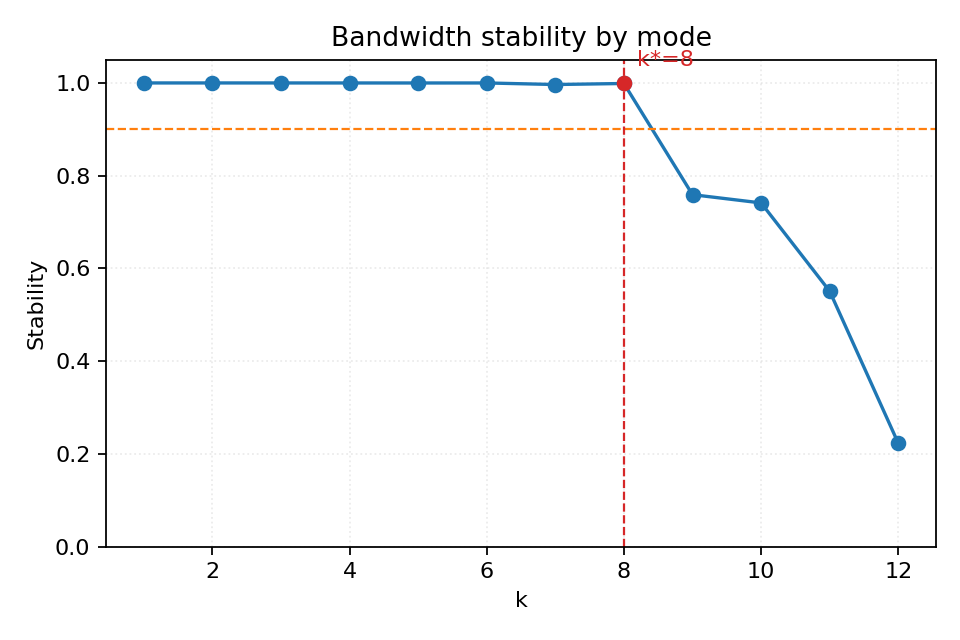
\includegraphics[width=\textwidth]{figures/stability_circle_r002.png}
    \caption{$r = 0.02$: signal--noise boundary at $k = 8$.}
\end{subfigure}
\hfill
\begin{subfigure}[b]{0.48\textwidth}
    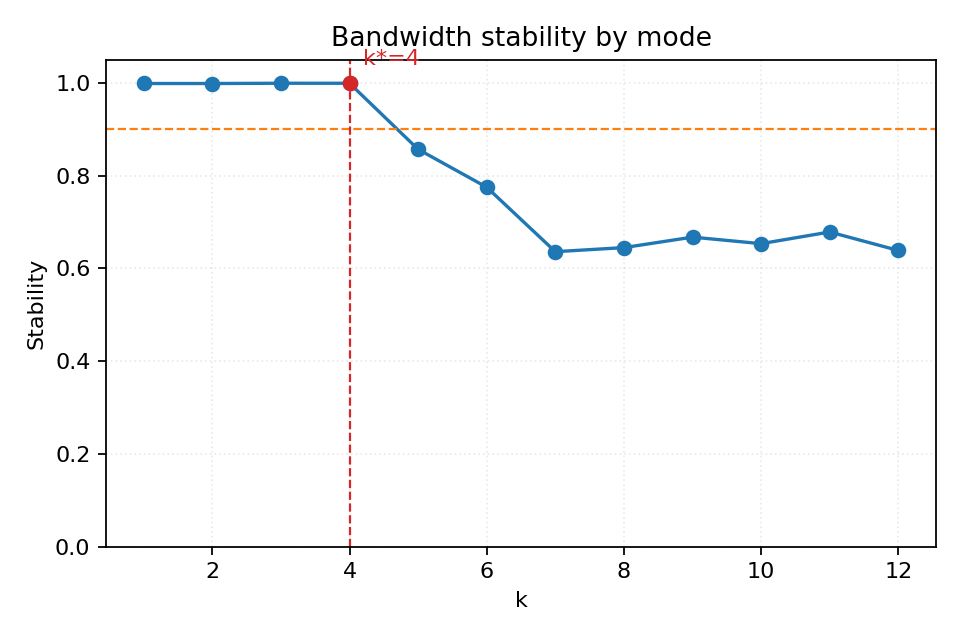
\includegraphics[width=\textwidth]{figures/stability_circle_r016.png}
    \caption{$r = 0.16$: boundary shifts to $k = 4$.}
\end{subfigure}
\caption{Stability scores for the circle at low and high noise. The sharp drop-off identifies the signal--noise transition. The dashed line marks $\tau = 0.9$.}
\label{fig:stability_circle}
\end{figure}

\begin{figure}[htbp]
\centering
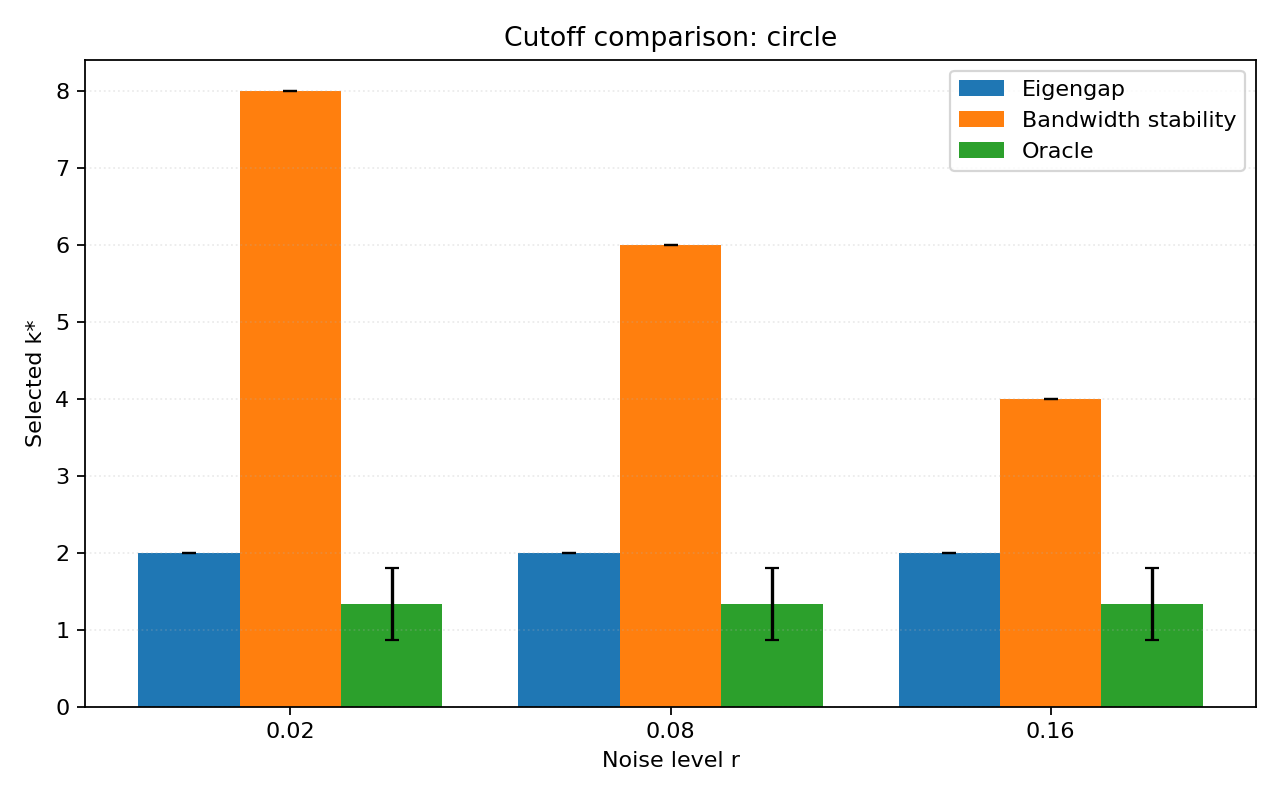
\includegraphics[width=0.65\textwidth]{figures/method_comparison_circle.png}
\caption{Cutoff comparison across noise levels for the circle. Bandwidth stability (blue) adapts monotonically; the eigengap (orange) is constant at $k = 2$; the oracle (green) is constant at $k \approx 1$.}
\label{fig:method_comparison_circle}
\end{figure}

\subsection{Sphere: Consistent Adaptation with Boundary Sensitivity}

On the sphere ($n = 450$, $D = 5$), the stability cutoff again decreases with noise: $k = 12 \to 10.7 \to 8$ (Table~\ref{tab:sphere_results}). At medium noise, one mode near the stability boundary causes slight seed variance ($k_{\text{stab}} = 10.7 \pm 1.2$): across the three seeds, the method selects $k = 10, 12, 10$. This is a realistic failure mode---near the threshold, the binary accept/reject decision is inherently sensitive to the specific noise realization. The low and high noise conditions have zero seed variance.

Geodesic consistency on the sphere (${\sim}0.44$) is lower than on the circle (${\sim}0.78$). This reflects the sphere's more complex geometry: geodesic distances on the sphere are harder to approximate from low-dimensional embeddings.

\begin{table}[htbp]
\caption{Sphere: full metrics across noise levels (3-seed means).}
\label{tab:sphere_results}
\centering
\begin{tabular}{@{}ccccccc@{}}
\toprule
$r$ & $k_{\text{stab}}$ ($\pm$std) & $k_{\text{gap}}$ & $k_{\text{oracle}}$ & Trust. & Cont. & Geo.\ cons. \\
\midrule
0.02 & 12.0 $\pm$ 0.0 & 3 & 1.7 & 0.855 & 0.440 & 0.442 \\
0.08 & 10.7 $\pm$ 1.2 & 3 & 1.7 & 0.854 & 0.403 & 0.435 \\
0.16 & 8.0 $\pm$ 0.0 & 3 & 1.7 & 0.853 & 0.320 & 0.415 \\
\bottomrule
\end{tabular}
\end{table}

\subsection{S-Curve: Outperforming the Eigengap on Ambiguous Spectra}

The S-curve experiment was designed per the professor's feedback to test whether the stability method finds the correct cutoff when the spectral gap is ambiguous. The S-curve has a gradual eigenvalue decay with no pronounced gap. As shown in Table~\ref{tab:scurve_results}, the eigengap collapses to $k = 1$---a trivially low value---while bandwidth stability retains 13 modes with $+3.5$ percentage points in trustworthiness and $+7.9$~pp in continuity. Both methods are seed-consistent on this manifold.

However, $k = 13$ seems high for a 2-dimensional manifold. Inspecting the stability profile, there is a dip at mode~10 (score 0.84) that recovers at mode~13 (score 0.91). The current rule---take the \emph{largest} $k$ above threshold---jumps over this dip. A ``first-drop'' rule that stops at the first mode below threshold would give $k = 9$, which may be more appropriate. This non-monotonic behavior reveals interesting spectral structure that a fixed threshold does not fully exploit.

\begin{table}[htbp]
\caption{S-curve ($r = 0.12$): method comparison. The eigengap fails on gradual-decay spectra.}
\label{tab:scurve_results}
\centering
\begin{tabular}{@{}lccc@{}}
\toprule
Method & $k^*$ ($\pm$std) & Trustworthiness & Continuity \\
\midrule
Eigengap & 1.0 $\pm$ 0.0 & 0.879 & 0.179 \\
Bandwidth stability & 13.0 $\pm$ 0.0 & 0.914 & 0.258 \\
\bottomrule
\end{tabular}
\end{table}

\subsection{Swiss Roll: Where Per-Vector Stability Fails}
\label{sec:swiss_roll_failure}

The Swiss roll is our main negative result. Across all experiments---single runs, noise sweeps ($r = 0.03, 0.08, 0.16$), and bandwidth sweeps (narrow and wide grids)---the stability method selects $k = 1$. Even with a narrow bandwidth grid ($2.2\times$ ratio from minimum to maximum $\varepsilon$), stability scores fail to reach $\tau = 0.9$ for any mode above $k = 1$.

The failure mechanism is specific and instructive. The Swiss roll has non-uniform curvature (a spiral). Small bandwidth perturbations cause eigenvectors to \emph{rotate} or \emph{reorder} within their eigenspace, destroying per-vector alignment even though the \emph{subspace} spanned by modes $1$--$k$ may be perfectly stable. On the circle and sphere, the eigenvectors correspond to Fourier modes and spherical harmonics, respectively---globally defined functions that are robust to bandwidth changes. On the Swiss roll, modes~2 and~3 can mix under small perturbations, which our per-vector dot-product metric registers as instability.

The eigengap also fails on the Swiss roll: across the noise sweep, $k_{\text{gap}}$ ranges from 1 to 3 across seeds, and geodesic consistency is consistently negative (${\sim}{-}1.97$), indicating that the embedding's distance structure is \emph{anti-correlated} with the manifold's geodesic structure at these parameter settings.

A subspace-based comparison using principal angles between $\mathrm{span}\{\psi_1, \ldots, \psi_k\}^{(a)}$ and $\mathrm{span}\{\psi_1, \ldots, \psi_k\}^{(b)}$ would be robust to intra-subspace rotations. The principal-angle computation exists in our codebase (\texttt{src/nase/metrics/subspace.py}), but we did not complete its integration into the cutoff selection path.

\subsection{Torus: Complex Stability Landscape}

The torus ($d = 2$, $D = 5$) shows less clean behavior than the circle or sphere: $k_{\text{stab}} = 8.7, 10.0, 8.7$ across noise levels with standard deviations of $2.1$--$2.9$. The torus has two independent circular dimensions, producing a richer eigenvalue spectrum and a more complex stability landscape where modes can be near the threshold boundary at multiple noise levels simultaneously. Trustworthiness remains consistently high (${\sim}0.96$) and geodesic consistency (${\sim}0.78$) is strong, indicating that the embedding captures the manifold structure even though the cutoff is less stable.

\subsection{Sphere in Higher Ambient Dimension: When the Eigengap Suffices}

On the sphere embedded in $\mathbb{R}^6$ with $r = 0.14$, the eigengap is perfectly stable ($k = 3$, zero variance across seeds) because the sphere's spectral gap after the first three spherical harmonics is pronounced even at this noise level. The stability method gives $k = 8$--$9$ with slight variance. This experiment demonstrates that the eigengap is not universally bad---it works well when the spectrum has a genuine cliff. The problem is manifolds where the cliff does not exist (S-curve) or does not adapt to noise (circle).

\subsection{Threshold Sensitivity}
\label{sec:threshold_sensitivity}

We tested four stability thresholds $\tau \in \{0.80, 0.85, 0.90, 0.95\}$ on the circle at $r = 0.08$ (Figure~\ref{fig:threshold_sensitivity}). The cutoff is $k = 6$ for $\tau \in \{0.85, 0.90, 0.95\}$ and $k = 6.33$ at $\tau = 0.80$. This insensitivity arises because stability scores drop sharply (from ${>}0.999$ to ${\sim}0.745$) at the signal--noise boundary, making the exact threshold irrelevant on this manifold. Only at $\tau = 0.80$ does one additional mode occasionally pass. This sharp transition is reassuring: it means the method is not highly sensitive to the threshold hyperparameter, at least on manifolds with clean spectral structure.

On the Swiss roll, however, $\tau$ would be decisive: lowering it below 0.9 might allow some modes through but would risk including noise. The threshold's effect is thus manifold-dependent, reflecting the sharpness of the stability drop-off.

\begin{figure}[htbp]
\centering
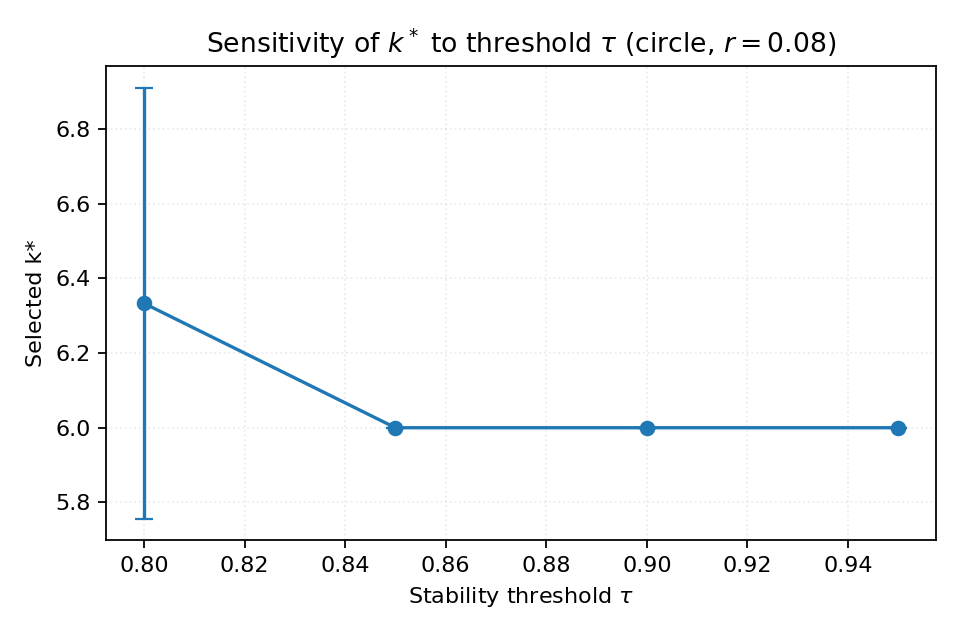
\includegraphics[width=0.50\textwidth]{figures/threshold_sensitivity.png}
\caption{Selected $k^*$ as a function of stability threshold $\tau$ for the circle at $r = 0.08$. The sharp spectral boundary makes the method insensitive to $\tau$ in the range $0.85$--$0.95$.}
\label{fig:threshold_sensitivity}
\end{figure}

\subsection{Oracle Subspace Distance Profiles}

To understand why the oracle consistently selects very low $k$ values ($k = 1$--$2$ across all conditions), we examined the subspace distance $d_{\text{sub}}(k)$ between clean and noisy eigenspaces as a function of $k$ (Figure~\ref{fig:oracle_profiles}). For both the circle and sphere, $d_{\text{sub}}$ is minimized at $k = 1$--$2$ and increases monotonically with $k$. Adding more noisy eigenvectors increases the mismatch with the clean eigenspace.

This reveals an important conceptual distinction: the oracle minimizes \emph{subspace distance from the clean eigenspace}, not embedding quality. A single well-aligned eigenvector produces a low subspace distance but yields a 1D embedding that discards too much structure for practical use. When we evaluate the oracle's chosen $k$ using trustworthiness and continuity (Table~\ref{tab:quality_at_k}), the oracle produces substantially worse embeddings than either the eigengap or bandwidth stability. The oracle criterion and downstream embedding quality measure fundamentally different things.

\begin{figure}[htbp]
\centering
\begin{subfigure}[b]{0.48\textwidth}
    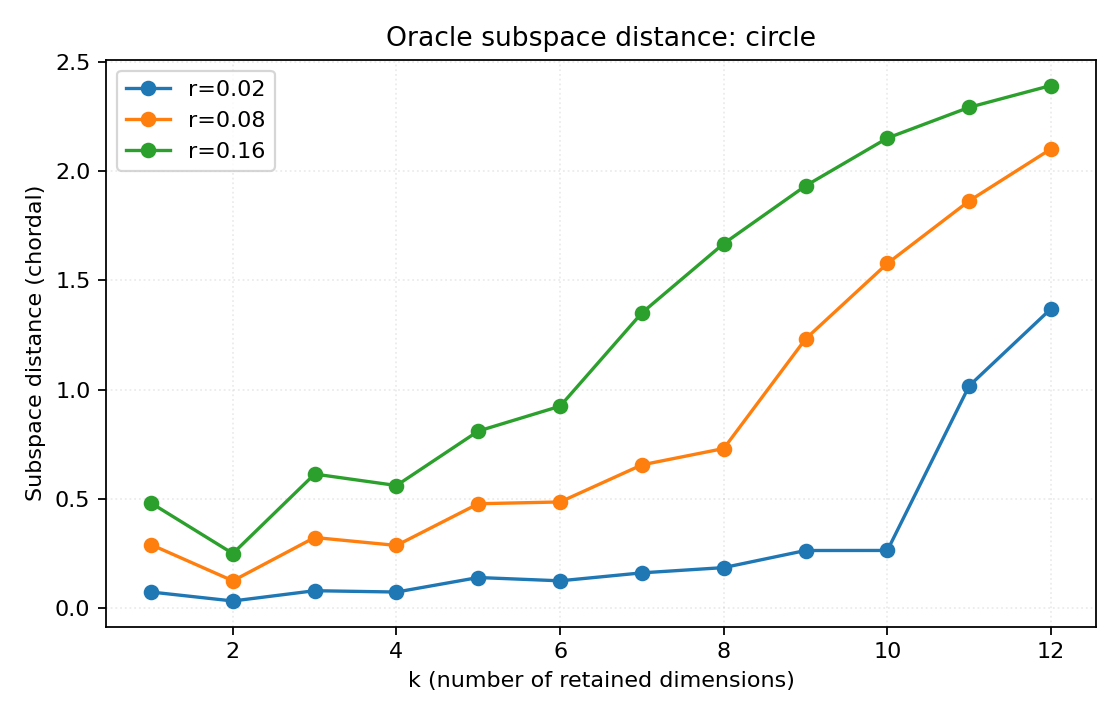
\includegraphics[width=\textwidth]{figures/oracle_subspace_profile_circle.png}
    \caption{Circle}
\end{subfigure}
\hfill
\begin{subfigure}[b]{0.48\textwidth}
    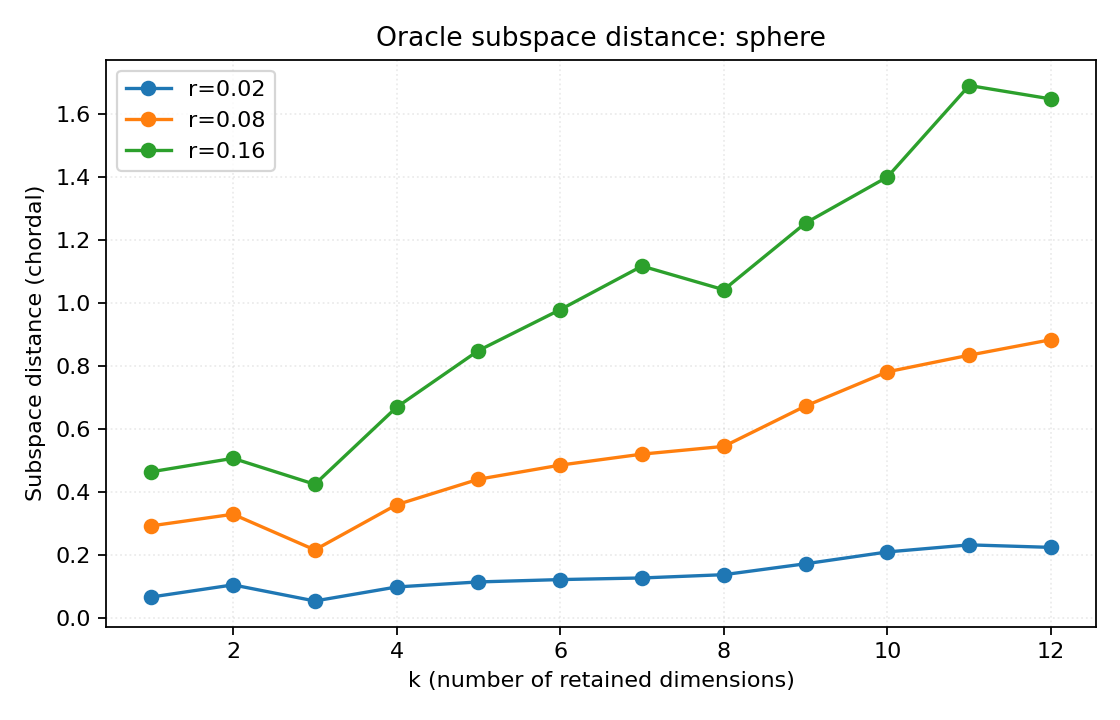
\includegraphics[width=\textwidth]{figures/oracle_subspace_profile_sphere.png}
    \caption{Sphere}
\end{subfigure}
\caption{Oracle subspace distance $d_{\text{sub}}(k)$ vs.\ retained dimensions $k$. The minimum at $k = 1$--$2$ explains the oracle's conservative selection.}
\label{fig:oracle_profiles}
\end{figure}

\begin{table}[htbp]
\caption{Embedding quality at each method's chosen $k$ (circle, 3-seed means). The oracle's conservative $k$ produces worse embeddings than either alternative.}
\label{tab:quality_at_k}
\centering
\begin{tabular}{@{}clcccc@{}}
\toprule
$r$ & Method & $k$ & Trust. & Cont. & Geo.\ cons. \\
\midrule
\multirow{3}{*}{0.02} & Eigengap & 2 & 0.9997 & 0.885 & 0.778 \\
 & Stability & 8 & 0.9997 & 0.885 & 0.778 \\
 & Oracle & ${\sim}1$ & 0.843 & 0.558 & 0.695 \\
\midrule
\multirow{3}{*}{0.16} & Eigengap & 2 & 0.981 & 0.453 & 0.746 \\
 & Stability & 4 & 0.981 & 0.453 & 0.746 \\
 & Oracle & ${\sim}1$ & 0.825 & 0.271 & 0.657 \\
\bottomrule
\end{tabular}
\end{table}

% ============================================================================
\clearpage
\section{Results: Noise Estimation and the \texorpdfstring{$r$}{r}-Based Cutoff}
\label{sec:noise_estimation}

\subsection{Intrinsic Dimension Estimation}

The Levina--Bickel estimator recovers the true intrinsic dimension within ${\sim}15\%$ on clean data: circle $\hat{d} = 1.15$ vs.\ $d = 1$; sphere $\hat{d} = 2.25$ vs.\ $d = 2$; Swiss roll $\hat{d} = 1.97$ vs.\ $d = 2$. Noise inflates the estimate because nearest-neighbor distances in noisy data include the noise contribution, making the data appear higher-dimensional. On the sphere, $\hat{d}$ increases from $2.42$ at $r = 0.02$ to $4.68$ at $r = 0.16$---more than double the true dimension. The Swiss roll estimate is relatively noise-robust ($2.01 \to 2.18$), likely because its 2D structure is well-separated in 3D ambient space.

The ceiling of the intrinsic dimension estimate, $\lceil \hat{d} \rceil$, provides a useful lower-bound reference for the truncation cutoff that is closer to the true manifold dimension than the bandwidth-stability selection, which tends to retain more modes than strictly necessary for recovering manifold coordinates.

\subsection{Validating the \texorpdfstring{$r^{-2}$}{1/r-squared} Scaling}

The noisy-Laplacian theory predicts $k_{\text{oracle}} \propto 1/r^2$. Using oracle data from all experiments, we computed the empirical constants $C = k_{\text{oracle}} \cdot r^2$ per manifold (Figure~\ref{fig:oracle_scaling}). The values are very small: $C \approx 0.014$ for the circle, $0.018$ for the sphere, $0.015$ for the torus, and effectively zero for the Swiss roll. The expected linear relationship between $k_{\text{oracle}}$ and $1/r^2$ is difficult to observe because $k_{\text{oracle}}$ is consistently 1--2 across all conditions at our sample sizes and noise ranges.

These small $C$ values have a practical consequence: the formula $k^* = C/r^2$ with $C \approx 0.015$ gives $k^* = 37$ at $r = 0.02$ (clipped to 12) but $k^* = 1$ at $r = 0.12$. The steep $1/r^2$ dependence means the formula transitions from ``keep everything'' to ``keep almost nothing'' over a narrow noise range.

\begin{figure}[htbp]
\centering
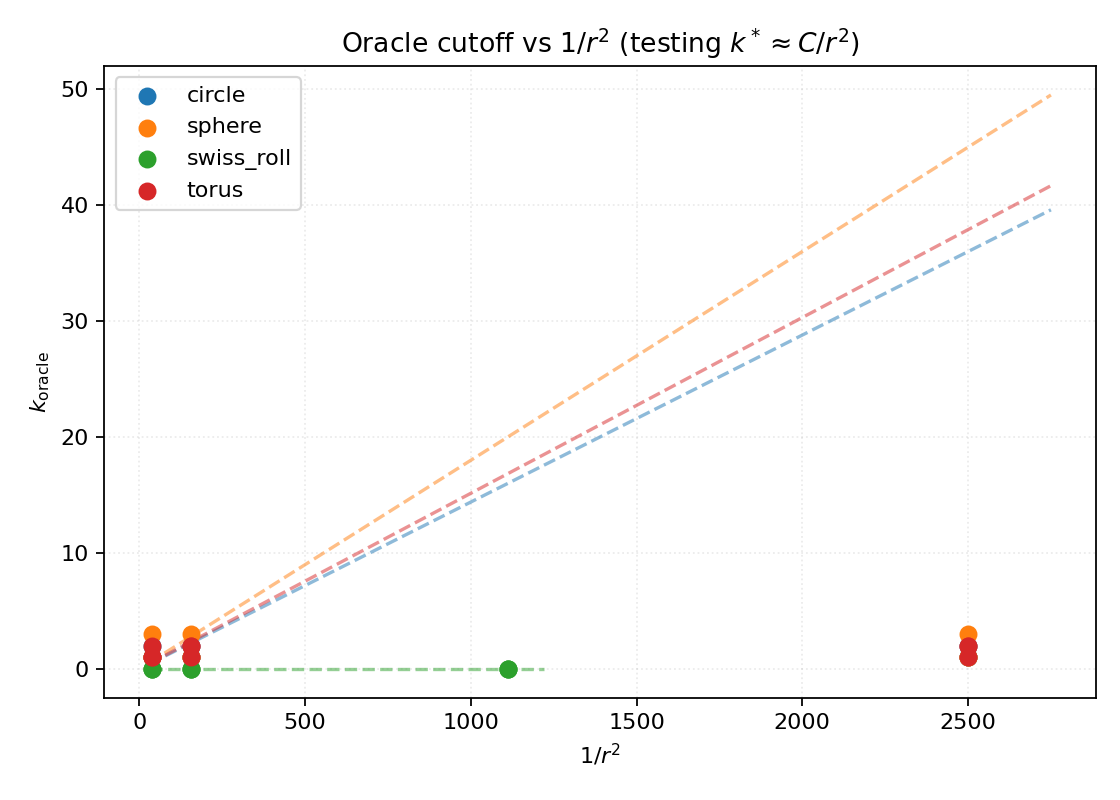
\includegraphics[width=0.55\textwidth]{figures/oracle_scaling.png}
\caption{Oracle cutoff $k^*$ vs.\ $1/r^2$ by manifold. The expected linear relationship is weak due to the oracle's conservative selection at our sample sizes.}
\label{fig:oracle_scaling}
\end{figure}

\subsection{Noise Amplitude Estimation Accuracy}
\label{sec:noise_amp_accuracy}

We evaluated both the simple and two-scale kNN noise estimators against the empirical noise amplitude computed directly from the known noise vectors (Section~\ref{sec:empirical_r_method}).

\paragraph{Empirical $r$ vs.\ configured $r$.} Across all 120 runs, $r_{\text{empirical}} / r_{\text{configured}}$ falls in $[0.976, 1.009]$, confirming that the finite-sample noise realization closely matches the target distribution (Figure~\ref{fig:empirical_r_comparison}, left). The tight agreement confirms that the entire gap between $r_{\text{empirical}}$ and $\hat{r}_{\text{kNN}}$ is attributable to estimator bias, not data-generation artifacts.

\paragraph{kNN estimates vs.\ empirical $r$.} The kNN estimators show systematic, manifold-dependent bias (Table~\ref{tab:r_estimation}, Figures~\ref{fig:empirical_r_comparison}--\ref{fig:knn_bias}):

\begin{table}[htbp]
\caption{kNN noise estimation accuracy: ratio of $\hat{r}_{\text{simple}}$ to $r_{\text{empirical}}$, averaged across seeds. Values below 1 indicate underestimation; above 1 indicate overestimation.}
\label{tab:r_estimation}
\centering
\begin{tabular}{@{}lcccccc@{}}
\toprule
& & \multicolumn{5}{c}{$\hat{r}_{\text{simple}} / r_{\text{empirical}}$} \\
\cmidrule(l){3-7}
Manifold & $D$ & $r{=}0.02$ & $r{=}0.05$ & $r{=}0.08$ & $r{=}0.12$ & $r{=}0.16$ \\
\midrule
Circle & 3 & $0.70\times$ & $0.49\times$ & $0.41\times$ & $0.36\times$ & $0.33\times$ \\
Sphere & 5 & $2.10\times$ & $1.07\times$ & $0.83\times$ & $0.68\times$ & $0.59\times$ \\
Swiss roll & 3 & $7.02\times$ & --- & $2.69\times$ & --- & $1.48\times$ \\
Torus & 5 & $3.50\times$ & --- & $1.14\times$ & --- & $0.77\times$ \\
\bottomrule
\end{tabular}
\end{table}

\begin{figure}[htbp]
\centering
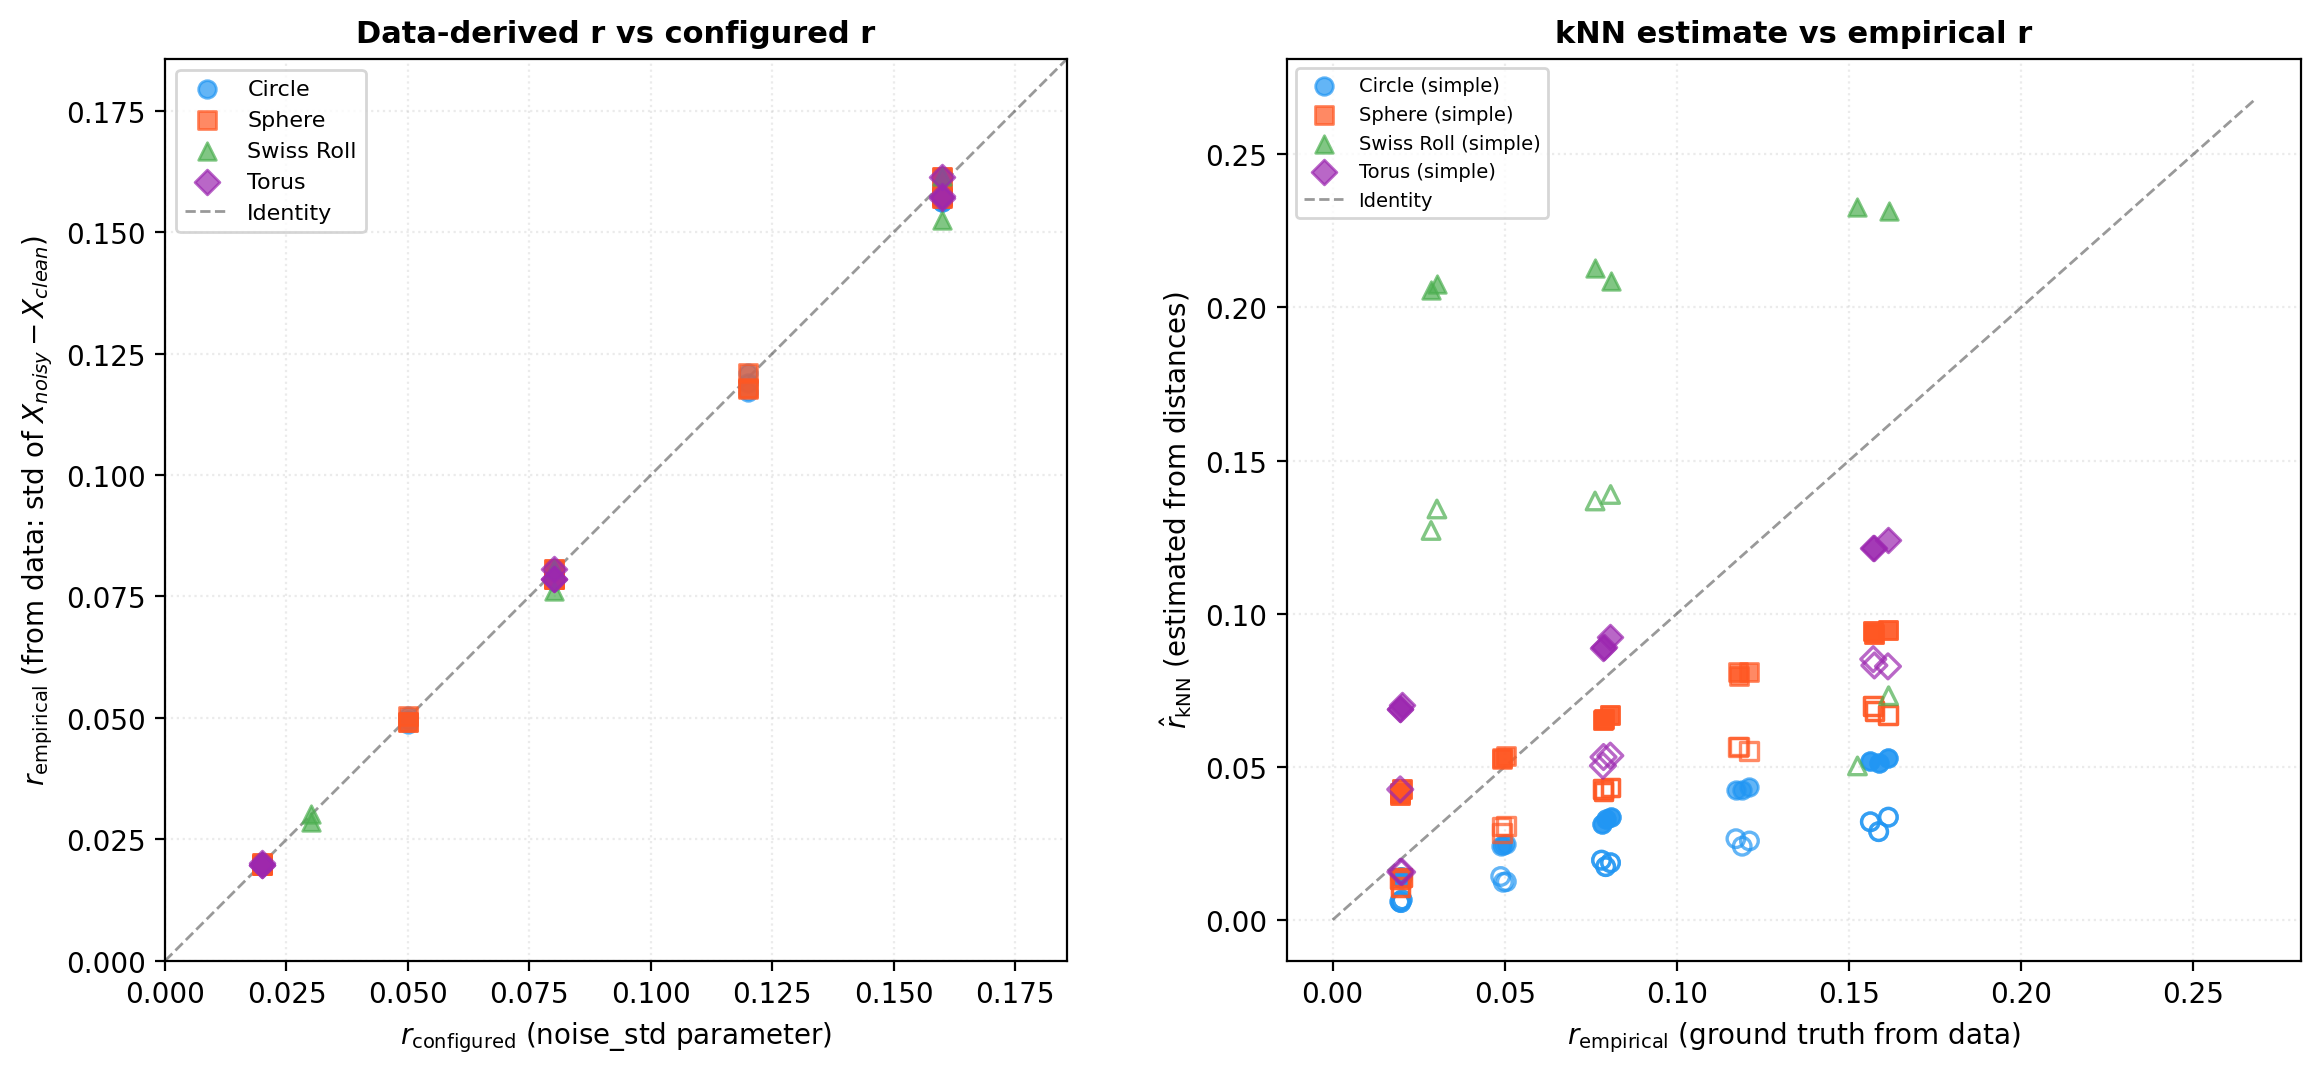
\includegraphics[width=0.95\textwidth]{figures/r_empirical_vs_configured_and_knn.png}
\caption{\textbf{Left:} $r_{\text{empirical}}$ vs.\ $r_{\text{configured}}$. Points lie on the identity line, confirming data generation accuracy. \textbf{Right:} kNN estimates vs.\ $r_{\text{empirical}}$. Filled markers show the simple estimator; open markers show the two-scale estimator. Deviation from the identity line quantifies estimation bias.}
\label{fig:empirical_r_comparison}
\end{figure}

\begin{figure}[htbp]
\centering
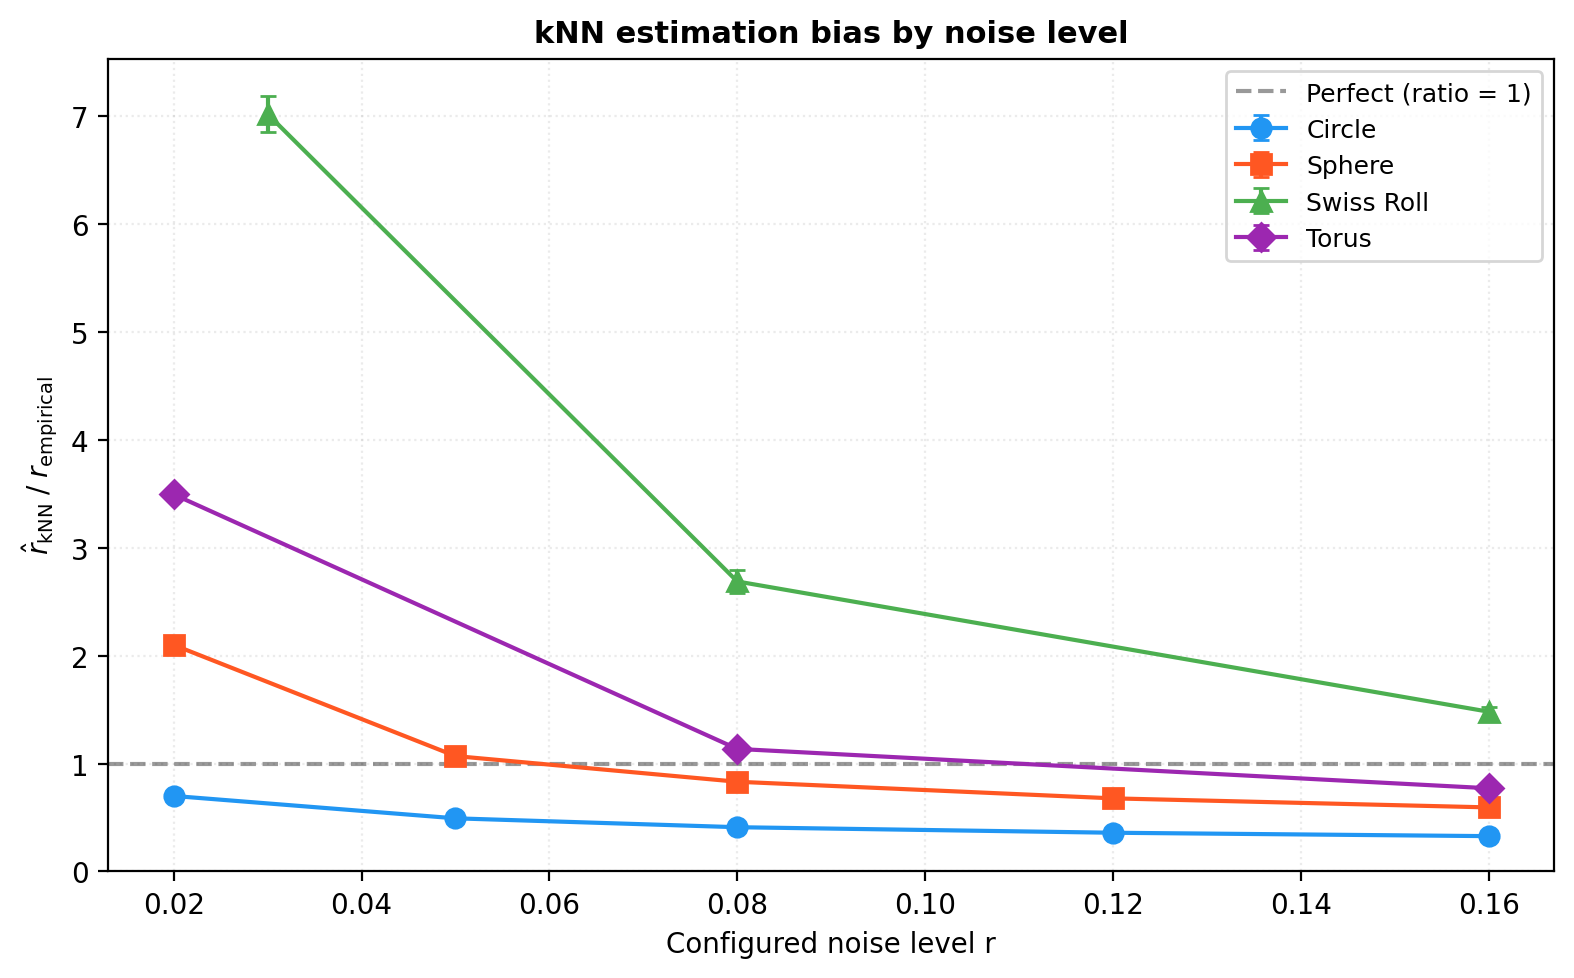
\includegraphics[width=0.55\textwidth]{figures/knn_estimation_bias_by_noise.png}
\caption{Ratio $\hat{r}_{\text{kNN}} / r_{\text{empirical}}$ across noise levels by manifold. The dashed line marks perfect estimation. The Swiss roll estimator returns ${\sim}0.21$ regardless of $r$.}
\label{fig:knn_bias}
\end{figure}

The estimation biases have clear geometric explanations:

\begin{enumerate}
    \item \textbf{Circle ($D = 3$, $d = 1$):} On a 1D curve in 3D, nearest-neighbor distances are dominated by the manifold arc length, not noise. The noise contribution to the total NN distance is small, so dividing by $2D$ in Eq.~\eqref{eq:simple_estimator} overcompensates. The estimator consistently underestimates $r$ by $30$--$70\%$, with the bias worsening at higher noise (where arc length exceeds the noise scale by a larger factor).

    \item \textbf{Sphere ($D = 5$, $d = 2$):} At low noise ($r = 0.02$), pairwise distances on the sphere surface are substantial even without noise, causing overestimation ($2.1\times$). As noise increases, the noise contribution becomes relatively more important, and the estimator transitions to underestimation ($0.59\times$ at $r = 0.16$). The crossover occurs near $r \approx 0.05$.

    \item \textbf{Swiss roll ($D = 3$, $d = 2$):} The spiral geometry means that nearest-neighbor distances along the manifold far exceed the noise contribution at all tested noise levels. The estimator returns $\hat{r} \approx 0.21$ regardless of whether $r_{\text{true}} = 0.03$ or $r_{\text{true}} = 0.16$, making it essentially uninformative.

    \item \textbf{Torus ($D = 5$, $d = 2$):} Follows the same crossover pattern as the sphere: overestimation at low noise ($3.5\times$), crossing to underestimation at high noise ($0.77\times$). The crossover occurs near $r \approx 0.08$.
\end{enumerate}

The two-scale estimator (Eq.~\eqref{eq:twoscale_estimator}) performs worse than the simple estimator across all manifolds, producing estimates that are $20$--$60\%$ of the true value. The heuristic assumption that the manifold contribution to $\mathbb{E}[d_k^2]$ scales linearly with neighborhood rank $k$ does not hold in practice.

\subsection{\texorpdfstring{$r$}{r}-Based Cutoff Performance}

Using the empirically calibrated constants ($C = 0.015$ for the circle, $C = 0.018$ for the sphere), we tested the formula $k^* = \lfloor C/r^2 \rfloor$ in both known-$r$ and estimated-$r$ modes (Table~\ref{tab:r_based_cutoff}, Figure~\ref{fig:r_based_comparison}).

\begin{table}[htbp]
\caption{Circle: $r$-based cutoff comparison. \emph{Est.}\ uses kNN-estimated $r$; \emph{Known} uses true $r$.}
\label{tab:r_based_cutoff}
\centering
\begin{tabular}{@{}cccccc@{}}
\toprule
$r_{\text{true}}$ & $k_{\text{r-est}}$ & $k_{\text{r-known}}$ & $k_{\text{stab}}$ & $k_{\text{gap}}$ & Trust. \\
\midrule
0.02 & 12 & 12 & 8 & 2 & 0.9997 \\
0.05 & 12 & --- & 6 & 2 & 0.997 \\
0.08 & 12 & 2 & 6 & 2 & 0.993 \\
0.12 & 8 & --- & 6 & 2 & 0.987 \\
0.16 & 5 & 1 & 4 & 2 & 0.981 \\
\bottomrule
\end{tabular}
\end{table}

\begin{figure}[htbp]
\centering
\begin{subfigure}[b]{0.48\textwidth}
    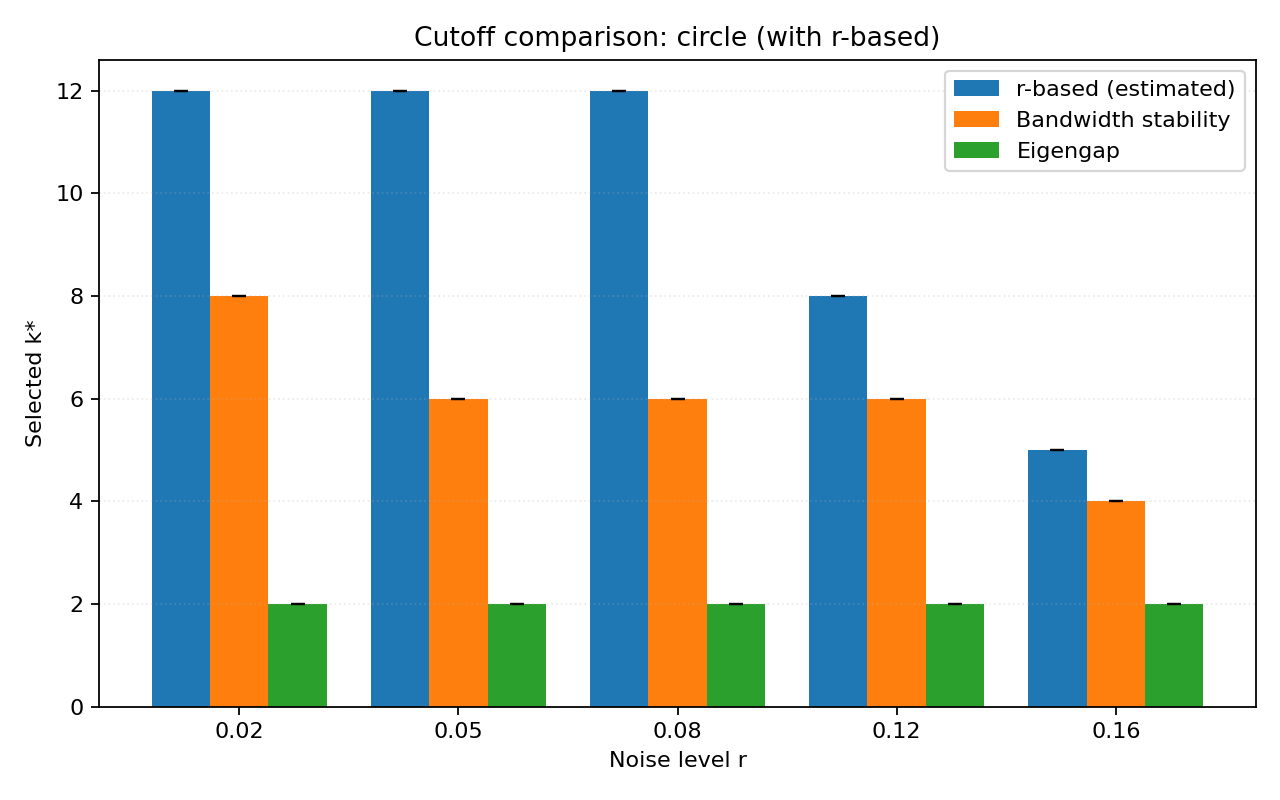
\includegraphics[width=\textwidth]{figures/r_based_comparison_circle.png}
    \caption{Circle}
\end{subfigure}
\hfill
\begin{subfigure}[b]{0.48\textwidth}
    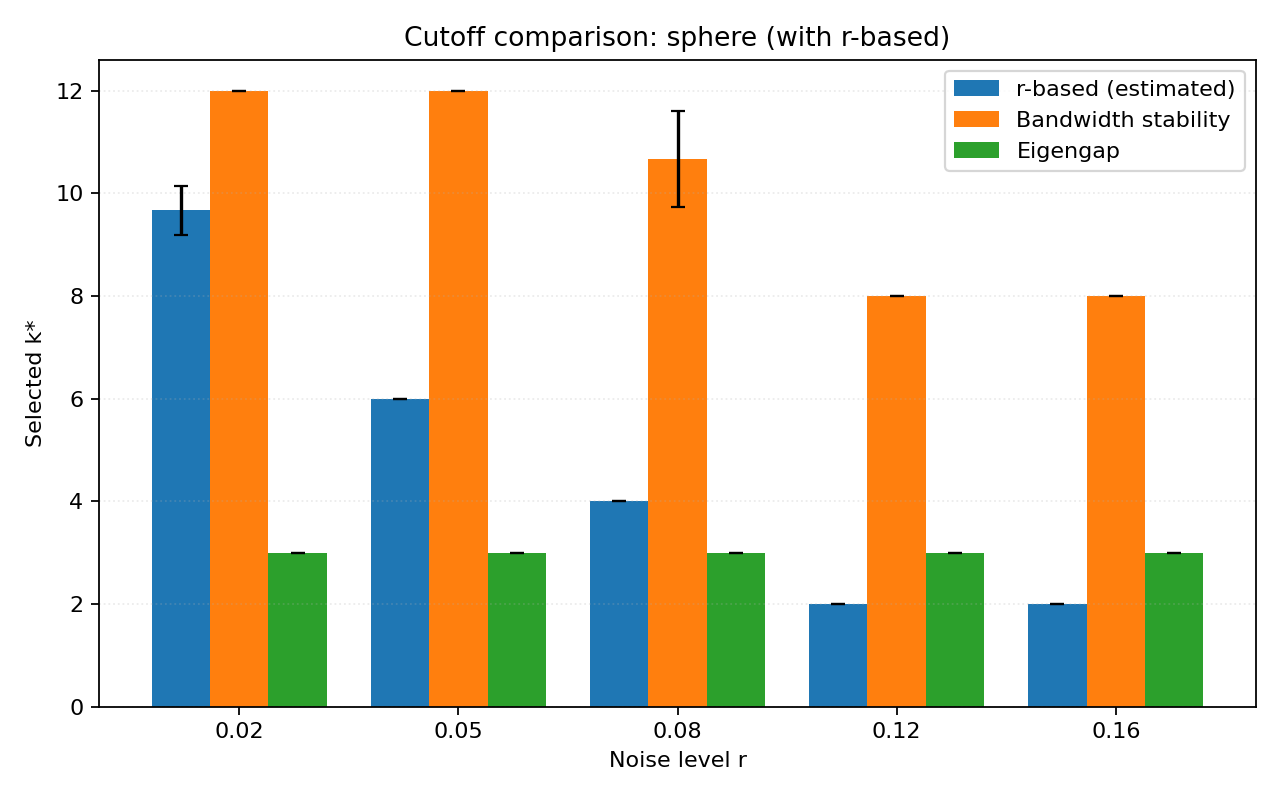
\includegraphics[width=\textwidth]{figures/r_based_comparison_sphere.png}
    \caption{Sphere}
\end{subfigure}
\caption{Cutoff comparison including the $r$-based method with estimated $r$.}
\label{fig:r_based_comparison}
\end{figure}

On the circle with estimated $r$, the cutoff decreases from 12 to 5 as noise increases from 0.02 to 0.16---qualitatively correct behavior. Ironically, the estimator's systematic underestimation of $r$ ($\hat{r} < r_{\text{true}}$) means $C/\hat{r}^2 > C/r_{\text{true}}^2$, partially compensating for the overly conservative $C$. This accidental cancellation produces reasonable cutoffs, but the mechanism is not reliable: it depends on the specific magnitude and direction of two independent biases.

With known $r$, the cutoff is too aggressive: $k = 12$ at $r = 0.02$ but drops to $k = 2$ at $r = 0.08$ and $k = 1$ at $r = 0.16$. This happens because $C = 0.015$ is so small that the formula predicts almost no signal modes at moderate noise. The issue is that $C$ was calibrated from the oracle, which itself selects very few modes (Section~\ref{sec:results_stability}).

On the sphere with estimated $r$, the cutoff decreases from 9.7 to 2.0, which is reasonable but substantially lower than bandwidth stability's $12 \to 8$. At $r = 0.12$ and $r = 0.16$, $k = 2$ may be too aggressive for producing useful embeddings.

% ============================================================================
\clearpage
\section{Discussion}
\label{sec:discussion}

\subsection{Bandwidth Stability as a Practical Truncation Rule}

The central question of this project was whether bandwidth stability can serve as a reliable, noise-adaptive truncation criterion for diffusion maps. Our experiments provide a nuanced answer: \emph{yes, on manifolds with uniform curvature, and no, on manifolds where eigenvectors reorder across bandwidths.}

The method's main strength is its ability to produce cutoffs that adapt to the noise level without requiring any knowledge of $r$ or $C$. On the circle, the stability cutoff tracks the noisy-Laplacian theory's prediction with remarkable fidelity: as noise increases $8\times$ (from $r = 0.02$ to $r = 0.16$), the cutoff decreases from $k = 8$ to $k = 4$ with \emph{zero variance across seeds}. The eigengap cannot do this---it always picks $k = 2$ regardless of noise, leaving information on the table at low noise levels. On the S-curve, where the eigengap collapses to $k = 1$ due to gradual spectral decay, bandwidth stability retains 13 modes and achieves meaningfully better embedding quality ($+3.5$~pp trustworthiness, $+7.9$~pp continuity). Both methods are seed-consistent on the S-curve, demonstrating that the instability of the eigengap on the Swiss roll is not a general sensitivity issue but rather a structural one: it depends on whether the spectrum has the sharp-gap structure the eigengap assumes.

The torus results are intermediate: the cutoff adapts to noise (decreasing from $8.7$ to $8.7$ with a non-monotonic peak at $10.0$ for medium noise) but with higher seed variance ($2.1$--$2.9$). The torus's two independent circular dimensions produce a richer spectrum than the circle or sphere, making the stability landscape more complex. Despite this, trustworthiness remains above 0.96 and geodesic consistency above 0.77 across all conditions.

\subsection{The Swiss Roll Failure: Per-Vector vs.\ Subspace Alignment}

The Swiss roll failure is the most instructive result of this project. The method measures stability by aligning \emph{individual} eigenvectors: $|\langle \psi_k^{(a)}, \psi_k^{(b)} \rangle|$. On the Swiss roll, even a small bandwidth change can cause eigenvectors to rotate within their eigenspace---for instance, modes 2 and 3 might mix---without the underlying signal quality degrading. This looks like instability to our per-vector metric even though the \emph{subspace} $\mathrm{span}\{\psi_1, \ldots, \psi_k\}$ is stable.

The fix is conceptually straightforward: replace per-vector dot products with a subspace distance metric such as the maximum principal angle between $\mathrm{span}\{\psi_1, \ldots, \psi_k\}^{(a)}$ and $\mathrm{span}\{\psi_1, \ldots, \psi_k\}^{(b)}$. This is invariant to rotations within the subspace and would only detect genuinely different subspaces. We have the principal-angle computation in our codebase and a placeholder for this approach (\texttt{adjacent\_subspace\_stability\_stub} in \texttt{bandwidth\_stability.py}), but did not complete the integration. This is the single highest-priority extension.

The circle and sphere do not exhibit this failure because their eigenvectors are globally defined (Fourier modes, spherical harmonics). On manifolds with simple, uniform curvature, per-vector alignment and subspace alignment are effectively equivalent.

\subsection{The Fundamental Difficulty of Noise Estimation}

Our kNN noise estimation experiments provide concrete empirical evidence for the theoretical difficulty anticipated in the course feedback. The core issue is Eq.~\eqref{eq:expected_distance}: nearest-neighbor distances contain \emph{both} noise and manifold contributions, and separating them requires knowing the manifold---which is precisely what we are trying to learn. This circular dependency manifests differently across manifold geometries:

On the circle ($d = 1$, $D = 3$), the 1D arc is densely sampled (450 points on a unit circle), so nearest-neighbor distances along the manifold are small but non-negligible compared to the noise. The estimator divides total NN distance by $2D = 6$, attributing too much to noise in the denominator. The result is systematic underestimation that worsens as noise increases (the manifold contribution remains constant while the noise grows, but the manifold contribution is never truly negligible at these sample sizes).

On the sphere and torus ($D = 5$), the higher ambient dimension means the $2D$ divisor is larger, while the manifold surface distances at the nearest-neighbor scale are also substantial. At low noise, the manifold distances dominate and the estimator overestimates $r$. At high noise, the noise term becomes the larger component, but the formula still attributes some manifold distance to noise, leading to underestimation. The crossover between these regimes depends on the specific manifold geometry.

The Swiss roll is the extreme case: its spiral structure means that even nearest neighbors on the manifold surface are separated by substantial distances (the spiral windings create large local spread). The estimator returns $\hat{r} \approx 0.21$ regardless of whether $r_{\text{true}} = 0.03$ or $0.16$, because the manifold contribution overwhelms the noise at all tested scales.

The empirical noise amplitude analysis (Section~\ref{sec:empirical_r_method}) strengthens these conclusions. By computing $r_{\text{empirical}} = \mathrm{std}(X_{\text{noisy}} - X_{\text{clean}})$ directly from the known noise vectors, we confirm that $r_{\text{empirical}} / r_{\text{configured}} \in [0.976, 1.009]$---the data generation is accurate and the entire estimation gap lies between $r_{\text{empirical}}$ and $\hat{r}_{\text{kNN}}$. This rules out the possibility that the bias is an artifact of the data generation process.

\subsection{Theory vs.\ Practice for the \texorpdfstring{$C/r^2$}{C/r-squared} Formula}

The theoretical formula $k^* = C/r^2$ is elegant but faces three compounding practical obstacles:

\begin{enumerate}
    \item \textbf{$C$ is tiny and hard to calibrate.} The empirical $C$ values (${\sim}0.015$) are very small, meaning the formula transitions from ``keep maximum modes'' to ``keep 1 mode'' over a narrow noise range. This steep dependence on $r$ makes the formula fragile: small errors in $r$ or $C$ cause large changes in $k^*$. Furthermore, $C$ was calibrated from oracle data (which itself is very conservative); in a real-world setting, $C$ would need to be estimated or transferred from similar manifolds.

    \item \textbf{The kNN noise estimator is systematically biased.} The direction and magnitude of bias depend on the manifold geometry (underestimation on the circle, overestimation on the Swiss roll), making it impossible to apply a single correction factor.

    \item \textbf{Error cancellation is accidental, not reliable.} On the circle, the estimator's underestimation of $r$ partially compensates for the conservative $C$, producing reasonable cutoffs. But this cancellation is manifold-dependent: on the sphere, both biases push in the same direction (overestimated $r$ with conservative $C$), producing cutoffs that are too small.
\end{enumerate}

Bandwidth stability avoids all three issues. It does not need $C$ (no geometry constant), does not need $r$ (no noise estimation), and directly probes which modes are signal vs.\ noise through their invariance to bandwidth perturbations. This confirms the course feedback's suggestion that bandwidth stability is a more practical alternative to direct noise estimation.

\subsection{Sensitivity to Hyperparameters}

\paragraph{Stability threshold $\tau$.} On the circle, $\tau$ has minimal impact because the stability transition is sharp (Section~\ref{sec:threshold_sensitivity}). On manifolds with less clean spectral structure (torus, Swiss roll), $\tau$ becomes more consequential. A principled alternative would be to detect the first significant \emph{drop} in stability scores---a ``stability gap'' heuristic analogous to the eigengap but operating in stability-score space.

\paragraph{Bandwidth grid.} The choice of $\varepsilon$-grid matters, particularly on the Swiss roll. The grid must span a range that captures meaningful bandwidth variation without exceeding the manifold's reach. Our experiments used hand-tuned grids; a fully automatic approach would set the grid as percentiles of the pairwise distance distribution.

\paragraph{kNN rank for noise estimation.} Using $k = 1$ or $k = 2$ for the nearest-neighbor distance in the noise estimator makes little practical difference; we used $k = 2$ throughout. The two-scale estimator's performance is not improved by varying $k_1$ and $k_2$.

% ============================================================================
\section{Limitations and Future Work}
\label{sec:limitations}

\paragraph{Per-vector alignment.} The Swiss roll failure is the primary algorithmic limitation. Replacing per-vector dot products with subspace-based stability (principal angles between the span of leading $k$ eigenvectors at different bandwidths) is the highest-priority extension and is implementable with existing code.

\paragraph{Adaptive bandwidth grids.} The $\varepsilon$-grid is currently hand-tuned per manifold. Using percentiles of the pairwise distance distribution (e.g., the 10th, 25th, 50th, and 75th percentiles) would make the method fully automatic and would adapt the grid to the data's intrinsic scale.

\paragraph{Stability-gap heuristic.} The S-curve's non-monotonic stability profile (a dip at mode~10 that recovers at mode~13) suggests that a fixed threshold misses relevant structure. Detecting the first significant drop in stability scores could be more principled.

\paragraph{Scale and dimensionality.} All experiments use $n \leq 500$ and $D \leq 6$. Larger samples would sharpen eigenvalue separation and potentially reveal the $r^{-2}$ scaling more clearly. Higher ambient dimensions could change the effective range of the $\varepsilon$-grid and the behavior of the kNN noise estimator.

\paragraph{Real data.} We tested only on synthetic manifolds with isotropic Gaussian noise. Real-world data introduces unknown intrinsic dimension, non-Gaussian and heteroscedastic noise, varying sampling density, and no oracle access. Candidates for real-data validation include single-cell RNA-seq (developmental trajectories), image patches (Klein bottle manifold), and MNIST digit classes.

\paragraph{Improved noise estimation.} More sophisticated approaches---random projection into low-dimensional subspaces before estimating $r$, or iterative refinement that alternates between manifold recovery and noise estimation---could reduce the bias of the kNN estimator and make the $r$-based formula more practical.

% ============================================================================
\section{Conclusion}
\label{sec:conclusion}

We implemented and evaluated a bandwidth-stability truncation rule for diffusion maps, following the suggestion to use eigenvector consistency across kernel bandwidths as a proxy for the signal--noise boundary. On five synthetic manifolds across 120 seeded experiments:

\begin{enumerate}
    \item \textbf{Bandwidth stability is noise-adaptive.} On the circle, $k$ decreases from 8 to 4 as noise increases eight-fold, with zero variance across seeds. On the S-curve, it outperforms the eigengap by $+3.5$~pp in trustworthiness when the spectrum has no clear gap.

    \item \textbf{Per-vector alignment fails on non-uniform curvature.} On the Swiss roll, eigenvectors reorder across bandwidths, collapsing the cutoff to $k = 1$. A subspace-based comparison would fix this.

    \item \textbf{kNN noise estimation is fundamentally biased by geometry.} The estimator underestimates $r$ on the circle ($0.3$--$0.7\times$), overestimates on the Swiss roll ($2$--$7\times$), and exhibits a dimension-dependent crossover on the sphere and torus. These biases are validated against the empirical noise amplitude computed directly from the known noise vectors.

    \item \textbf{The formula $k^* = C/r^2$ is elegant but fragile.} The empirically calibrated $C$ is very small (${\sim}0.015$), and the composition of biased $C$ and biased $\hat{r}$ can accidentally produce reasonable cutoffs but is not reliable as a general method.
\end{enumerate}

The project validates that bandwidth stability is a viable practical alternative to direct noise estimation for spectral truncation, while also providing concrete empirical evidence for why noise estimation from nearest-neighbor distances is fundamentally difficult---confirming the theoretical predictions that motivated this alternative approach.

% ============================================================================
\begin{ack}
This project was conducted for DSC~205 (Winter 2026) at the University of California, San Diego. We thank the course instructor for detailed feedback on the project proposal, particularly the suggestion to use bandwidth stability as a practical alternative to noise estimation and the warning about kNN-based noise estimation being biased by manifold geometry. Both observations directly shaped the project's direction and are empirically validated in this report.
\end{ack}

% ============================================================================
\bibliographystyle{plainnat}
\bibliography{references}

% ============================================================================
\newpage
\appendix

\section{Notation Reference}
\label{app:notation}

\begin{table}[htbp]
\centering
\begin{tabular}{@{}cl@{}}
\toprule
Symbol & Meaning \\
\midrule
$n$ & Number of data points \\
$D$ & Ambient dimension \\
$d$ & Intrinsic manifold dimension \\
$r$ & Noise standard deviation (additive Gaussian) \\
$\hat{r}$ & Estimated noise standard deviation \\
$r_{\text{empirical}}$ & Noise std computed from $X_{\text{noisy}} - X_{\text{clean}}$ \\
$\varepsilon$ & Kernel bandwidth \\
$\alpha$ & Anisotropic normalization parameter ($= 0.5$) \\
$t$ & Diffusion time \\
$k$ & Number of non-trivial eigenvectors retained \\
$k^*$ & Selected cutoff \\
$\tau$ & Stability threshold (default $0.9$) \\
$C(\mathcal{M})$ & Geometry-dependent constant (reach, curvature) \\
\bottomrule
\end{tabular}
\end{table}

\section{Additional Quality Metrics and Comparisons}
\label{app:quality_metrics}

\begin{figure}[htbp]
\centering
\begin{subfigure}[b]{0.48\textwidth}
    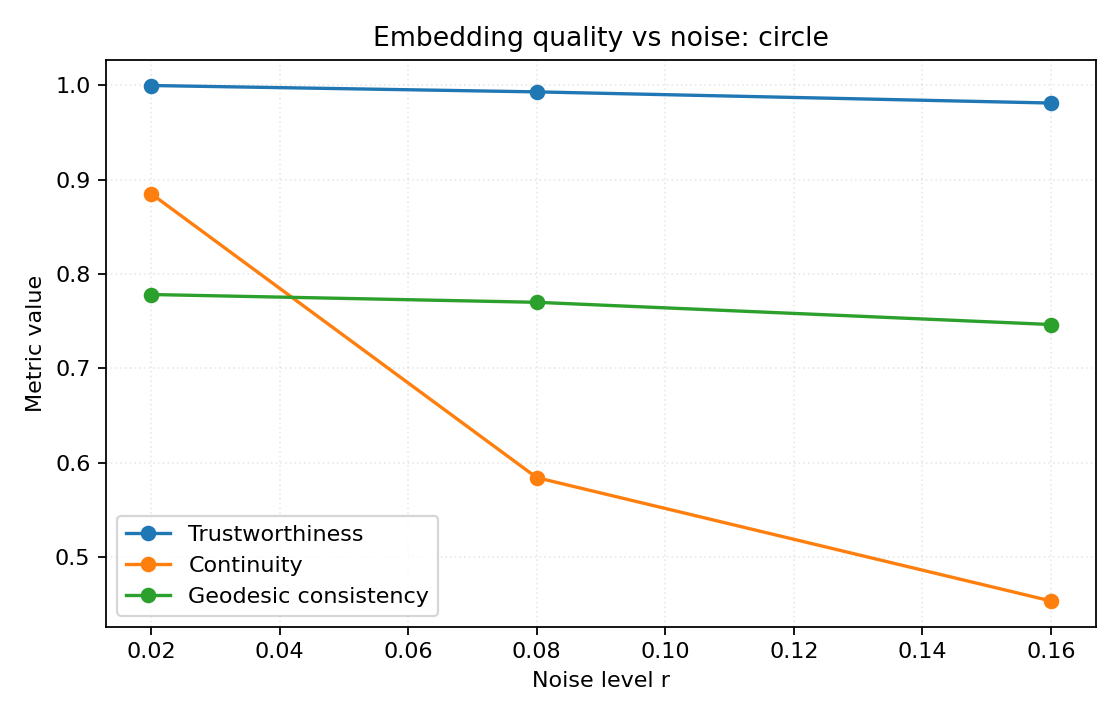
\includegraphics[width=\textwidth]{figures/quality_metrics_circle.png}
    \caption{Circle}
\end{subfigure}
\hfill
\begin{subfigure}[b]{0.48\textwidth}
    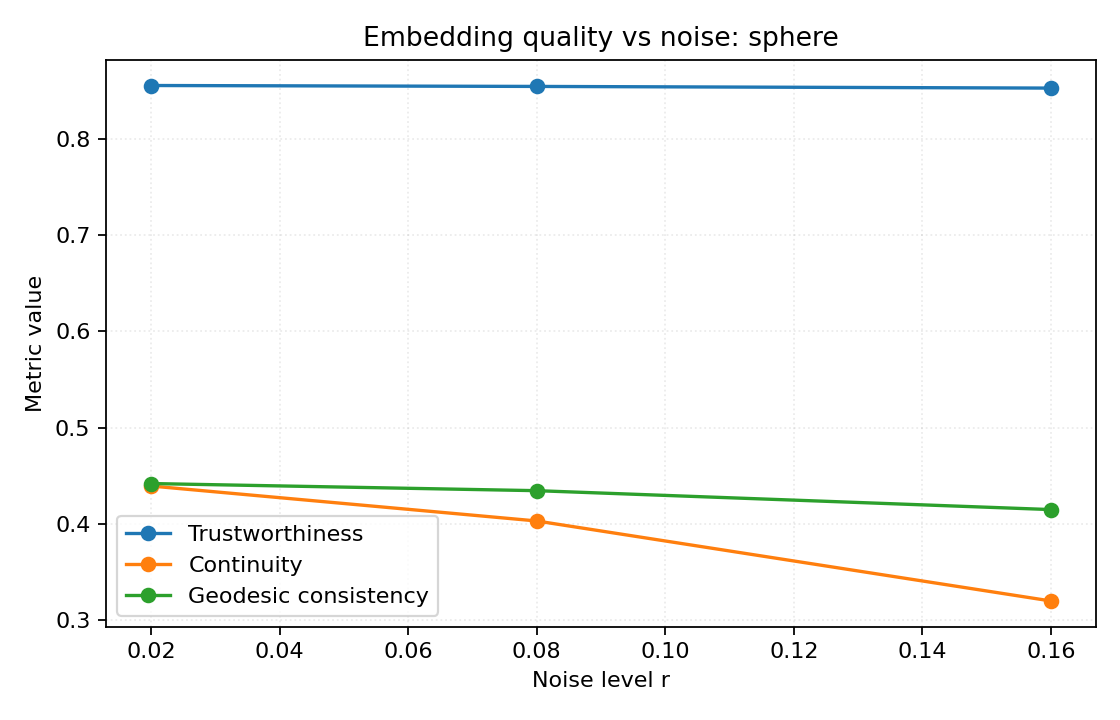
\includegraphics[width=\textwidth]{figures/quality_metrics_sphere.png}
    \caption{Sphere}
\end{subfigure}
\caption{Embedding quality metrics (trustworthiness, continuity, geodesic consistency) as a function of noise level for the circle and sphere.}
\label{fig:quality_metrics}
\end{figure}

\begin{figure}[htbp]
\centering
\begin{subfigure}[b]{0.48\textwidth}
    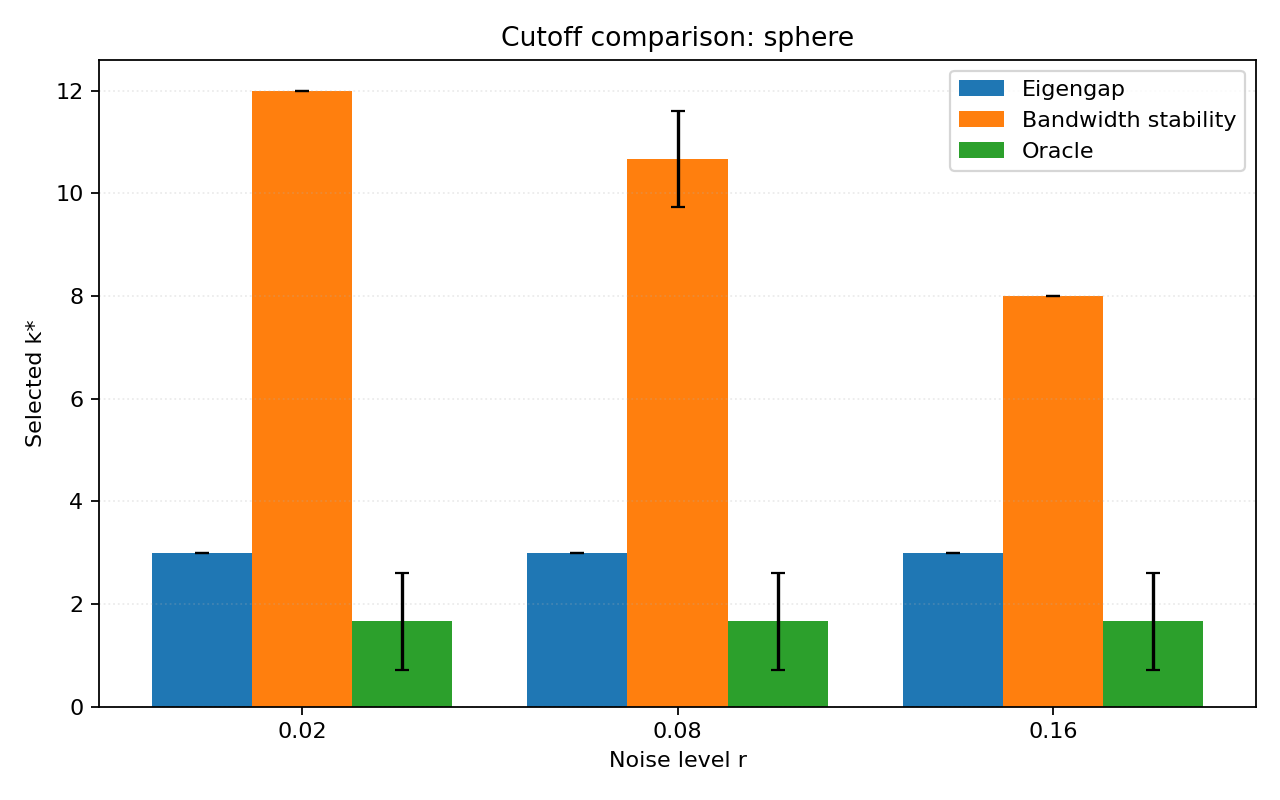
\includegraphics[width=\textwidth]{figures/method_comparison_sphere.png}
    \caption{Sphere}
\end{subfigure}
\hfill
\begin{subfigure}[b]{0.48\textwidth}
    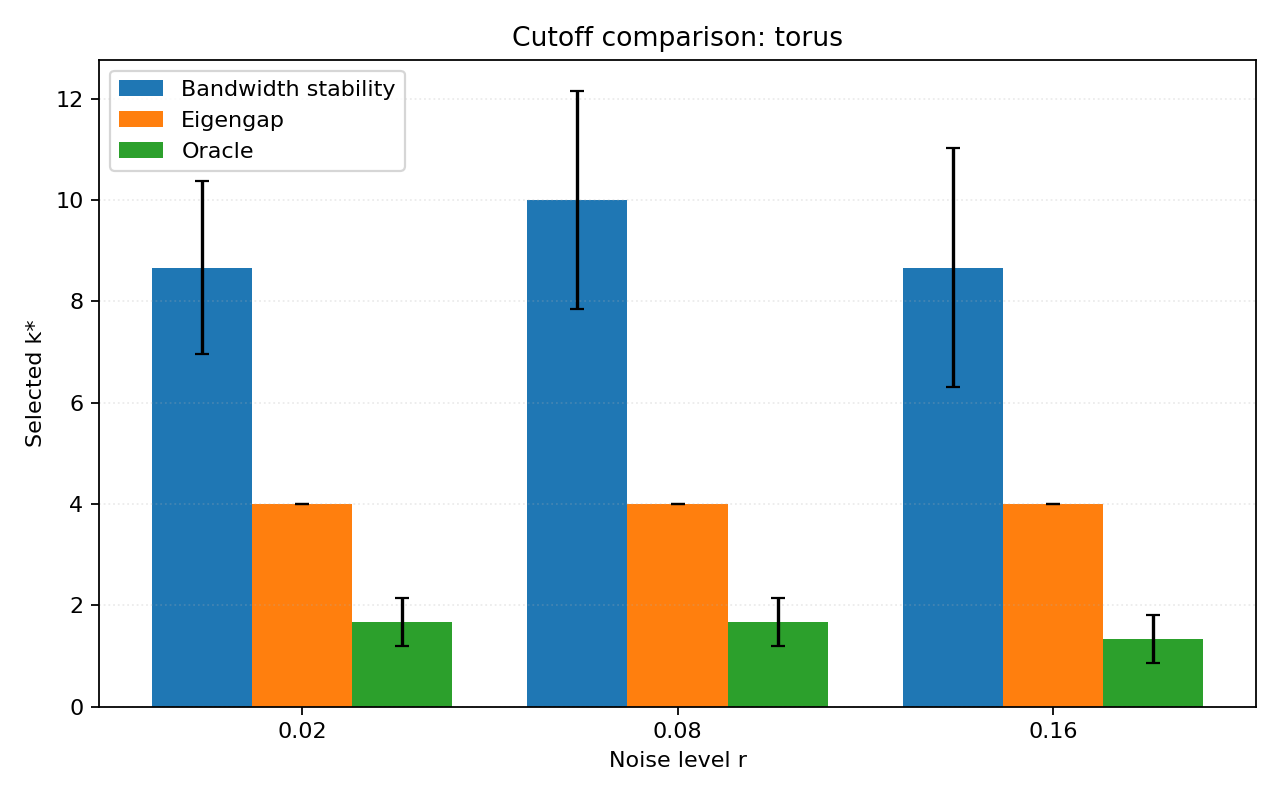
\includegraphics[width=\textwidth]{figures/method_comparison_torus.png}
    \caption{Torus}
\end{subfigure}
\caption{Cutoff comparison across noise levels for the sphere and torus.}
\label{fig:method_comparison_additional}
\end{figure}

\section{Noise Estimation: Scatter Plots}
\label{app:r_estimation_scatter}

\begin{figure}[htbp]
\centering
\begin{subfigure}[b]{0.48\textwidth}
    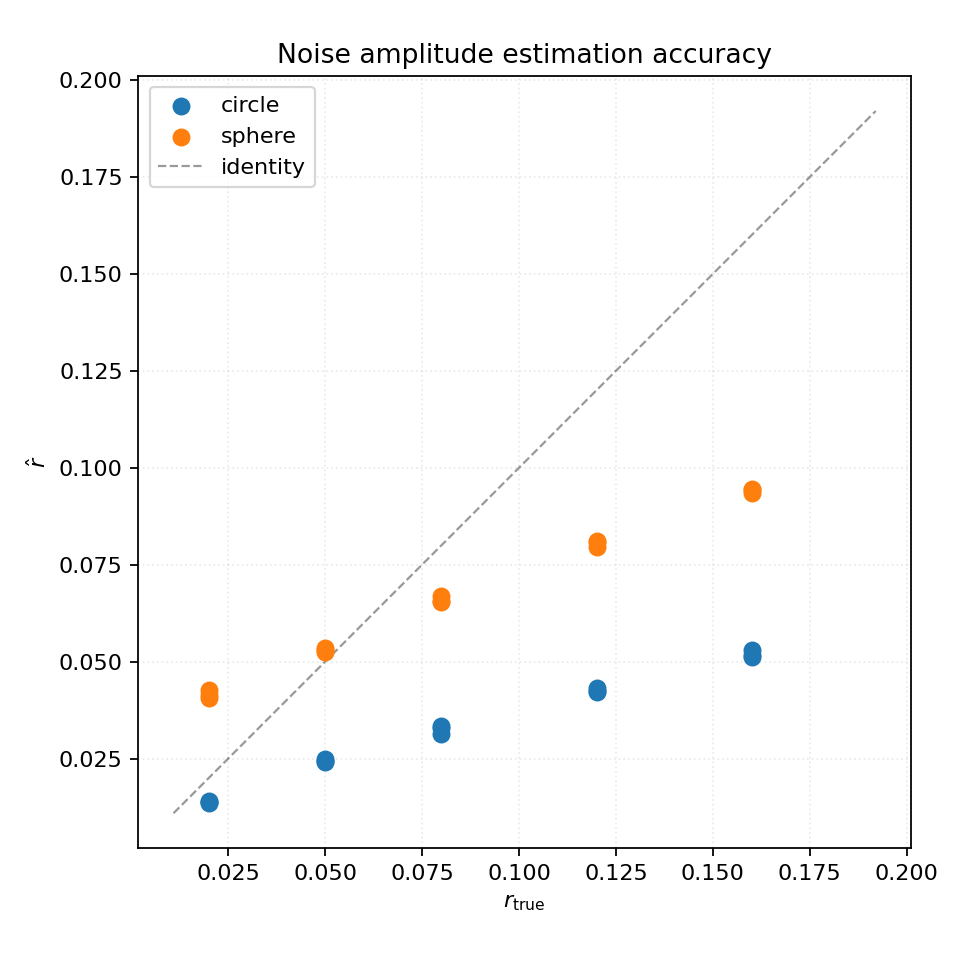
\includegraphics[width=\textwidth]{figures/r_estimation_simple.png}
    \caption{Simple estimator $\hat{r}_{\text{simple}}$ vs.\ $r_{\text{true}}$.}
\end{subfigure}
\hfill
\begin{subfigure}[b]{0.48\textwidth}
    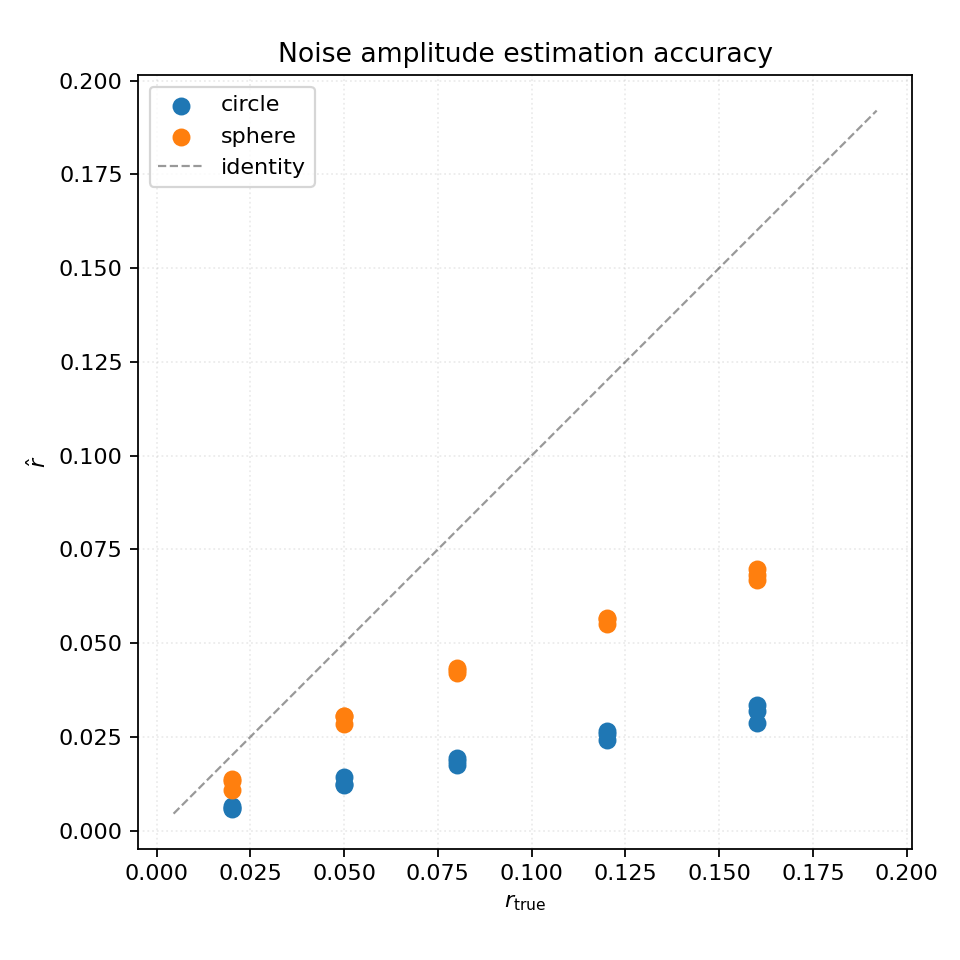
\includegraphics[width=\textwidth]{figures/r_estimation_twoscale.png}
    \caption{Two-scale estimator $\hat{r}_{\text{2-scale}}$ vs.\ $r_{\text{true}}$.}
\end{subfigure}
\caption{Noise amplitude estimation accuracy for both estimator variants. The simple estimator underestimates on the circle and overestimates at low noise on the sphere. The two-scale estimator exhibits more severe underestimation across both manifolds.}
\label{fig:r_estimation_scatter}
\end{figure}

\section{Spectral and Embedding Visualizations}
\label{app:spectral}

\begin{figure}[htbp]
\centering
\begin{subfigure}[b]{0.48\textwidth}
    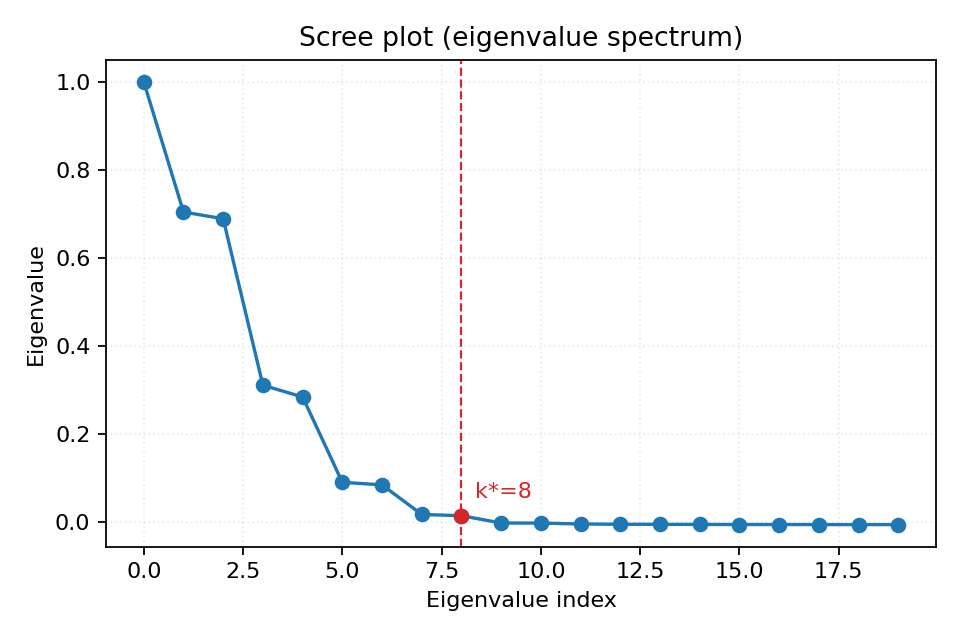
\includegraphics[width=\textwidth]{figures/spectrum_circle_r002.png}
    \caption{Eigenvalue spectrum at $r = 0.02$.}
\end{subfigure}
\hfill
\begin{subfigure}[b]{0.48\textwidth}
    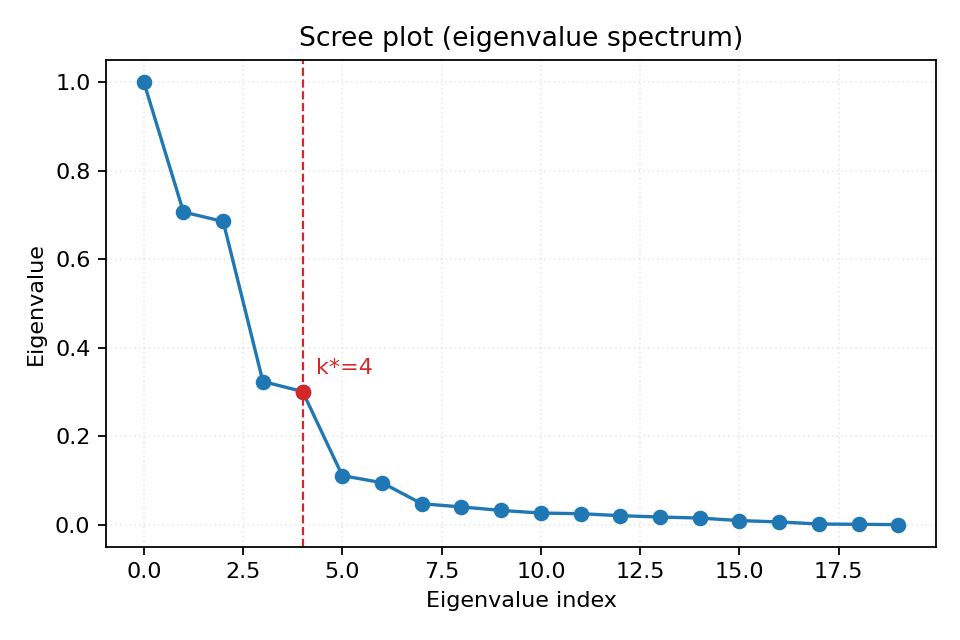
\includegraphics[width=\textwidth]{figures/spectrum_circle_r016.png}
    \caption{Eigenvalue spectrum at $r = 0.16$.}
\end{subfigure}

\vspace{4mm}

\begin{subfigure}[b]{0.48\textwidth}
    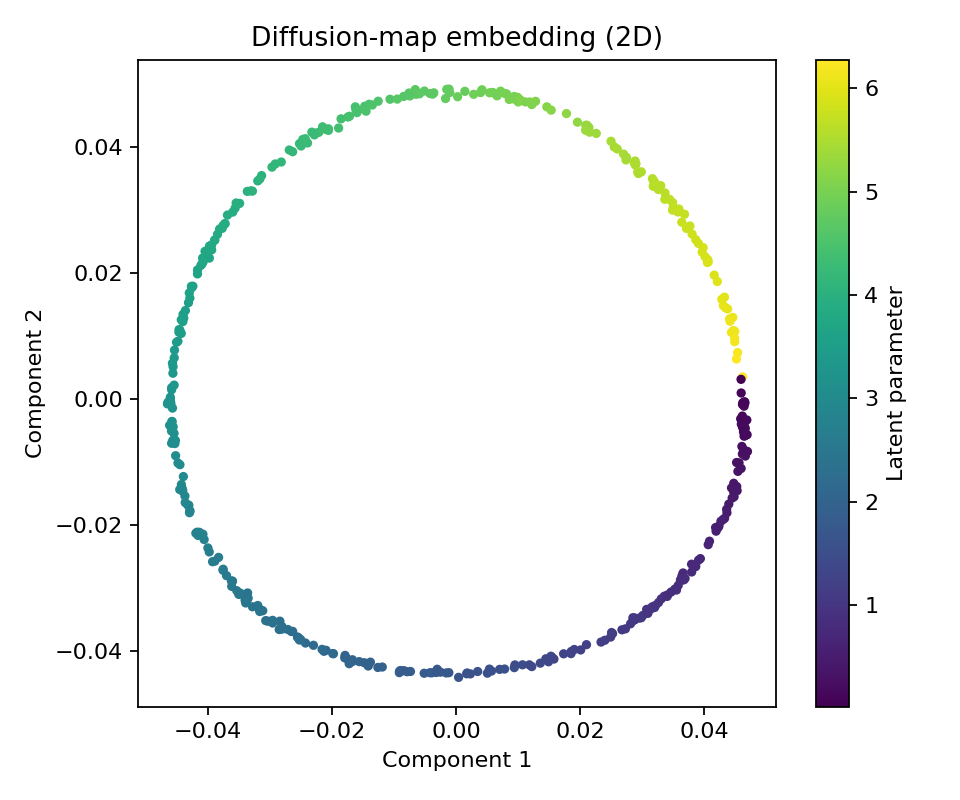
\includegraphics[width=\textwidth]{figures/embedding_circle_r002.png}
    \caption{2D embedding at $r = 0.02$.}
\end{subfigure}
\hfill
\begin{subfigure}[b]{0.48\textwidth}
    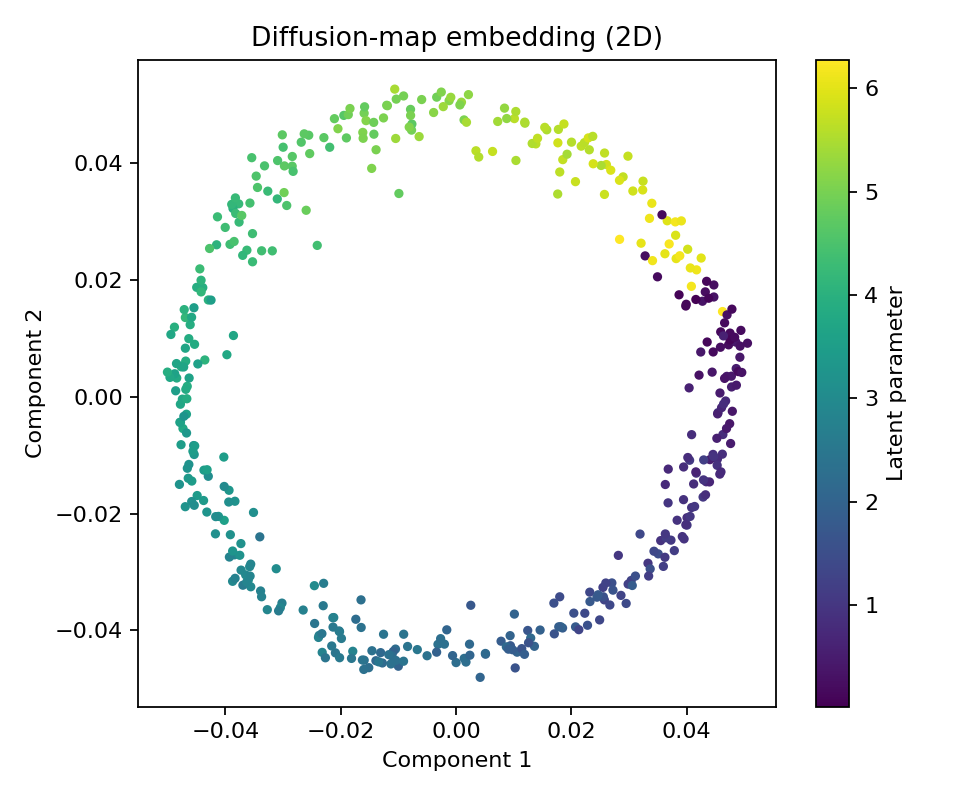
\includegraphics[width=\textwidth]{figures/embedding_circle_r016.png}
    \caption{2D embedding at $r = 0.16$.}
\end{subfigure}
\caption{Circle: eigenvalue spectra and diffusion-map embeddings at low and high noise. At $r = 0.02$, the embedding cleanly recovers a circular structure. At $r = 0.16$, the embedding is noisier but the circular topology is still visible.}
\label{fig:spectral_embedding}
\end{figure}

\end{document}
